
\documentclass[11pt,a4paper]{article}
\usepackage[margin=1in]{geometry}
\usepackage[utf8]{inputenc}
\usepackage[T1]{fontenc}
\usepackage{lmodern}
\usepackage{microtype}
\usepackage{array}
\usepackage{tabularx}
\usepackage{longtable}
\usepackage[table]{xcolor}
\usepackage{booktabs}
\usepackage{enumitem}
\usepackage{hyperref}
\usepackage{graphicx}
\usepackage{adjustbox}
\usepackage{pdflscape}
\usepackage{fancyhdr}
\usepackage{lastpage}
\usepackage{tikz}
\usetikzlibrary{arrows.meta,positioning,shapes.geometric,shapes.symbols,fit,calc,chains,decorations.pathreplacing,backgrounds}
\hypersetup{colorlinks=true, linkcolor=blue, urlcolor=blue, citecolor=blue}
\setlist[itemize]{leftmargin=*, itemsep=2pt, topsep=3pt}
\setlist[enumerate]{leftmargin=*, itemsep=2pt, topsep=3pt}
\renewcommand{\arraystretch}{1.15}
\setlength{\LTpre}{4pt}
\setlength{\LTpost}{6pt}
\sloppy
\emergencystretch=3em
\setlength{\headheight}{14pt}
\pagestyle{fancy}
\fancyhf{}
\lhead{Mudarabah-Enabled Procurement Network SRS}
\rhead{Version 1.1}
\cfoot{Page \thepage\ of \pageref{LastPage}}

\newcommand{\systemname}{Mudarabah-Enabled Procurement Network}
\newcommand{\systemshort}{MEPN}
\newcommand{\must}{\textbf{shall}}
\newcommand{\shouldword}{\textbf{should}}
\newcommand{\mayword}{\textbf{may}}
\newcommand{\code}[1]{\texttt{#1}}

\tikzset{
  actor/.style={draw, ellipse, minimum width=2.8cm, minimum height=0.8cm, align=center, fill=gray!8},
  usecase/.style={draw, ellipse, minimum width=3.2cm, minimum height=1.0cm, align=center, fill=blue!6, font=\scriptsize},
  usecasebig/.style={draw, ellipse, minimum width=4.1cm, minimum height=1.0cm, align=center, fill=blue!6, font=\scriptsize},
  act/.style={draw, rounded corners, text width=3.5cm, minimum height=0.8cm, align=center, fill=gray!8, font=\scriptsize},
  decision/.style={draw, diamond, aspect=2.2, text width=2.5cm, align=center, fill=orange!10, font=\scriptsize},
  ext/.style={draw, rounded corners, text width=3.2cm, minimum height=0.8cm, align=center, fill=green!8, font=\scriptsize},
  datastore/.style={draw, cylinder, shape border rotate=90, aspect=0.25, text width=2.8cm, align=center, fill=yellow!10, font=\scriptsize},
  arrow/.style={-{Latex[length=2mm]}, thick},
  dashedarrow/.style={-{Latex[length=2mm]}, thick, dashed},
  classbox/.style={draw, rectangle, rounded corners, text width=3.2cm, align=left, fill=gray!5, font=\scriptsize, minimum height=1.0cm},
  state/.style={draw, rounded corners, minimum width=3.4cm, minimum height=0.9cm, align=center, fill=blue!5, font=\scriptsize},
  seqnode/.style={draw, rounded corners, align=center, fill=gray!8, minimum width=2.7cm, minimum height=0.65cm, font=\scriptsize},
  lifeline/.style={densely dashed, gray},
  msg/.style={-{Latex[length=2mm]}, thick, font=\scriptsize},
  returnmsg/.style={-{Latex[length=2mm]}, thick, dashed, font=\scriptsize}
}

\begin{document}
\begin{titlepage}
\centering
\vspace*{1.0cm}
{\Large Software Requirements Specification\\[0.4cm]}
{\huge \textbf{Mudarabah-Enabled Distributed E-Procurement System}\\[0.35cm]}
{\Large Product codename: \systemshort{}\\[0.8cm]}
\vspace{0.8cm}
\begin{tabular}{ll}
Document status: & FYP review baseline aligned with current implementation evidence \\
Version: & 1.1 \\
Date: & 7 June 2026 \\
Prepared for: & SME organizations and financial entities \\
Primary standard alignment: & ISO/IEC/IEEE 29148:2011 SRS information item \\
UML package: & Use case, activity, class, state machine, external sequence, RTM \\
\end{tabular}
\vfill
\begin{minipage}{0.86\textwidth}
\small
This specification defines software requirements for a distributed e-procurement platform that automates procurement workflows and enables project-based mudarabah capital participation by banks, Islamic financial institutions, venture capital firms, or other approved financial entities. It is a tailored requirements artifact, not a legal contract, Shariah ruling, or production security assessment. Final use requires legal, Shariah, accounting, data protection, and regulatory review.
\end{minipage}
\vfill
\end{titlepage}

\pagenumbering{roman}
\tableofcontents
\listoffigures
\listoftables
\clearpage
\pagenumbering{arabic}

\section{Document Control and Tailoring Statement}

\subsection{Document identification}
\begin{table}[h]
\centering
\begin{tabularx}{\textwidth}{@{}lX@{}}
\toprule
Title & Software Requirements Specification for the Mudarabah-Enabled Distributed E-Procurement System \\
Revision & Version 1.1, 7 June 2026 \\
System of interest & \systemname{} (\systemshort{}) \\
Document type & Software Requirements Specification with UML appendices and traceability matrix \\
Intended readers & Product owner, software architects, developers, QA engineers, SME operators, financial entity stakeholders, Shariah/compliance reviewers, implementation partners \\
\bottomrule
\end{tabularx}
\caption{Document identification}
\end{table}

\subsection{Tailoring to ISO/IEC/IEEE 29148}
This SRS follows the 29148 information-item approach for a software requirements specification: purpose, scope, product overview, references, external interfaces, functional requirements, usability, performance, logical data, design constraints, software quality attributes, verification, assumptions, and acronyms. Additional stakeholder context, operational concept, UML models, and a traceability matrix are included because the product combines workflow automation, inter-organization collaboration, and regulated financing interactions.

The words \must{}, \shouldword{}, and \mayword{} are used deliberately. Only statements using \must{} are binding requirements in this document. Descriptive, architectural, or rationale statements are non-binding unless explicitly written as requirements.

\subsection{Source basis}
The requirements are derived from the product vision in the prompt, the uploaded Malaysia mudarabah performance report, the uploaded procurement and mudarabah-procurement thesis documents, the uploaded ISO/IEC/IEEE 29148 standard, the referenced ERPNext repository, official protocol references for OAuth/OpenID Connect and Hyperledger Fabric, and the current MEPN implementation/evidence baseline recorded in the roadmap, final validation matrix, and evidence index. The repository is used as the current implementation baseline for Version 1.1, while this SRS remains the behavioral source of truth.

\subsection{Current implementation and review boundary}
Version 1.1 tailors the original requirements to the implemented FYP review package. The current implementation includes a protected web application shell, role-based navigation, API-backed dashboard/procurement/finance summaries, procurement and restricted mudarabah review workflows, loss exception handling, audited report exports, graph risk/saved-view support, Fabric hash anchoring and chaincode verification, operator-assisted Fabric consortium governance, operations status/timeline visibility, PostgreSQL backup/restore proof, accessibility automation, and reviewer evidence documentation.

The current implementation is suitable for academic review, local validation, and Azure Student VM demonstration. It is not a regulated production financial deployment. Production OIDC provider UAT, PDF/spreadsheet report packs, object-storage backup automation, manual screen-reader/mobile accessibility review, real external ERP/e-signature/payment integrations, and fully automated Fabric topology administration remain product-hardening work.

\section{Introduction}

\subsection{Purpose}
The purpose of this SRS is to specify the required behavior, interfaces, data model, constraints, quality attributes, verification approach, and UML-supported analysis model for \systemshort{}. The system is intended to make mudarabah financing more commercially adoptable by embedding financiers into high-integrity procurement workflows, reducing information asymmetry, improving project-level accounting evidence, and providing auditable cross-organization records.

\subsection{Scope}
\systemshort{} is a distributed, self-hostable e-procurement and procurement-finance platform for SME organizations and financial entities. It supports conventional procurement automation, SME-to-SME business interaction, ERP integration, supply-chain network visibility, and restricted project-based mudarabah financing workflows.

\subsubsection{In scope}
\begin{itemize}
  \item Organization setup, organization profile/branding, user management, authorization, and role-based access control.
  \item Supplier onboarding, supplier master data, due diligence evidence, and supplier performance records.
  \item Source-to-contract functions: RFQ/RFP/tender publication, quotation management, evaluation, award, and contract record generation.
  \item Procure-to-pay functions: purchase requisition, approval, purchase order, goods receipt/service confirmation, invoice submission, three-way matching, payment status, and audit evidence.
  \item Procurement opportunity publication for revenue-generating trades, projects, resale cycles, or contract fulfillment.
  \item Mudarabah capital application, financier due diligence, Shariah/compliance review, contract execution, disbursement control, milestone monitoring, profit/loss calculation, profit distribution, and loss exception handling.
  \item Distributed deployment for SME-owned nodes with optional consortium participation through Hyperledger Fabric channels and operator-assisted channel governance.
  \item Supply-chain network graph/canvas showing organizations, supplier/customer relationships, opportunities, financing links, document status, risk indicators, saved views, and annotations where authorized.
  \item ERP integration through APIs, file exchange, and adapter services.
  \item Audit trail, immutable event anchoring, Fabric chaincode verification, evidence package browsing, report export, and operations evidence.
\end{itemize}

\subsubsection{Out of scope for version 1.0}
\begin{itemize}
  \item Full banking core replacement, deposit account management, or capital adequacy computation.
  \item Automated legal enforceability determination or automated Shariah rulings without human reviewer approval.
  \item Public permissionless blockchain settlement or crypto-token issuance.
  \item General consumer purchases that do not generate separately measurable project profit.
  \item Autonomous credit approval without financier-defined policies and accountable human approval.
  \item Production regulatory reporting formats not yet specified by a target regulator.
  \item Fully automated Fabric channel creation, peer join, MSP enrollment, channel configuration signing, or endorsement-policy mutation by the MEPN application.
  \item Production use of the demo/development login path or unverified mock integration data as real business evidence.
\end{itemize}

\subsection{Product perspective}
\systemshort{} is a distributed business application inspired by ERPNext's integrated ERP pattern. ERPNext exposes major ERP functions such as accounting, order management, manufacturing, asset management, and projects; the referenced repository also highlights a full-stack framework with database abstraction, user authentication, and REST API support, plus self-hosted Docker-oriented deployment. \systemshort{} adopts the integration breadth and self-hostability pattern, but rewrites the system as a modular distributed procurement-finance platform.

\subsection{Product functions}
At a high level, \systemshort{} provides the following product functions:
\begin{enumerate}
  \item Automate procurement workflows from need identification to payment reconciliation.
  \item Convert procurement documents into trusted financing evidence for project-based mudarabah.
  \item Allow financial entities to review, approve, monitor, and close mudarabah-backed procurement ventures.
  \item Provide distributed inter-organization visibility while preserving private business data.
  \item Anchor critical inter-organization events on Hyperledger Fabric channels for tamper-evident auditability.
  \item Integrate with SME ERP/accounting systems without requiring SMEs to surrender ownership of their deployment.
  \item Visualize supply chain relationships and financing dependencies through a canvas-style network interface.
\end{enumerate}

\subsection{User characteristics}
\begin{table}[h]
\centering
\begin{tabularx}{\textwidth}{@{}lX@{}}
\toprule
User class & Expected characteristics \\
\midrule
SME Owner/Admin & Manages installation, users, organization profile, integration settings, and network participation. May have limited IT staff. \\
Procurement Officer & Creates requisitions, RFQs, POs, receipts, supplier records, and financing evidence packs. Familiar with P2P/S2C workflows. \\
Approver/Manager & Reviews business justification, budget, supplier selection, purchase orders, and financing requests. Needs fast decision support. \\
Supplier/Sales User & Responds to RFQs, acknowledges POs, submits delivery documents and invoices, and views payment status. \\
Finance/Accountant & Reconciles invoices, payments, project accounts, allowable costs, profit/loss calculations, and ERP postings. \\
Financial Entity Investment Officer & Evaluates opportunity quality, project economics, risk, and contract terms before capital commitment. \\
Shariah/Compliance Reviewer & Checks goods/services eligibility, contract form, profit ratio, loss treatment, documentation, and compliance exceptions. \\
Auditor & Reviews evidence, event logs, Fabric transaction hashes, user actions, changes, and contract closure packages. \\
Developer/Integrator & Builds adapters, chaincode integration, deployment automation, and custom extensions. \\
\bottomrule
\end{tabularx}
\caption{User characteristics}
\end{table}

\subsection{Limitations}
\begin{itemize}
  \item Mudarabah commercial adoption depends on legal enforceability, financier appetite, Shariah governance, accounting discipline, and regulatory constraints that software can support but not eliminate.
  \item Hyperledger Fabric is used for audit anchoring and inter-organization coordination, not as the full transactional database for confidential procurement records.
  \item Financial entities remain responsible for underwriting, suitability checks, liquidity treatment, contract approval, and regulatory obligations.
  \item SMEs remain responsible for accurate records, lawful procurement, tax compliance, delivery performance, and truthful profit/loss reporting.
\end{itemize}

\subsection{Definitions}
\begin{description}[leftmargin=4.2cm, style=nextline]
  \item[Mudarabah] A partnership in which a capital provider supplies capital and a manager/operator deploys effort and expertise. Profit is shared by pre-agreed ratio; genuine financial loss is borne by capital unless negligence, misconduct, fraud, or breach is proven.
  \item[Rabb-ul-Mal] Capital provider in a mudarabah arrangement; in this product it is usually a financial entity.
  \item[Mudarib] Entrepreneur or procurement operator that uses capital to fulfill a procurement opportunity.
  \item[Restricted mudarabah] A mudarabah arrangement restricted to a specified project, purpose, expense category, supplier set, buyer contract, and reporting regime.
  \item[P2P] Procure-to-pay: need, requisition, approval, purchase order, receipt, invoice verification, and payment.
  \item[S2C] Source-to-contract: requirement definition, sourcing, RFQ/RFP/tender, evaluation, award, and contract record.
  \item[Three-way match] Control that reconciles purchase order, receipt/service confirmation, and supplier invoice.
  \item[Network canvas] Visual graph of organizations, suppliers, buyers, financing links, documents, risks, and status flows.
  \item[Fabric channel] Permissioned Hyperledger Fabric administrative and ledger domain shared by selected organizations.
  \item[Fabric Gateway verification] Verification mode in which MEPN queries approved chaincode, such as \code{ReadAnchor}, and compares the on-chain hash with local canonical hash and stored anchor metadata.
  \item[Operator-assisted Fabric governance] A governance workflow where MEPN records channel proposals, invitations, approvals, readiness checks, and sanitized execution evidence, while a Fabric operator executes topology changes outside the application.
\end{description}

\section{References}
\begin{thebibliography}{99}
\bibitem{iso29148} ISO/IEC/IEEE 29148:2011, \textit{Systems and software engineering - Life cycle processes - Requirements engineering}.
\bibitem{mudarabahperf} \textit{Mudarabah Performance Research Report - Malaysia}, uploaded research synthesis, May 2026.
\bibitem{mudproc} \textit{Understanding the Link between Mudarabah and Procurement}, uploaded conceptual thesis, 27 May 2026.
\bibitem{procthesis} \textit{Inefficiencies in Traditional Procurement and the Performance Impact of Digital Procurement Solutions}, uploaded evidence review, May 2026.
\bibitem{erpnextrepo} raichiiiiiii/erpnext GitHub repository, default branch \code{develop}, README and source files inspected 2 June 2026.
\bibitem{oauth} RFC 6749, \textit{The OAuth 2.0 Authorization Framework}, IETF/RFC Editor.
\bibitem{oidc} OpenID Foundation, \textit{OpenID Connect Core 1.0 incorporating errata set 2}.
\bibitem{fabric} Hyperledger Fabric Documentation, release 2.5, network, private data, MSP, and chaincode documentation.
\bibitem{featurestatus} \textit{MEPN Feature Status and Future Implementation Plan}, repository document \code{docs/roadmap/feature-status-and-future-implementation.md}, current review baseline.
\bibitem{evidenceindex} \textit{MEPN Evidence Index}, repository document \code{docs/evidence/EVIDENCE_INDEX.md}, current review evidence entry point.
\bibitem{fabricgovernance} \textit{Fabric Consortium Governance Requirements And Base Decision}, repository document \code{docs/roadmap/fabric-consortium-governance-requirements.md}.
\end{thebibliography}

\section{Business and Stakeholder Context}

\subsection{Business problem}
Traditional procurement frequently suffers from manual handoffs, fragmented data, weak controls, slow approvals, invoice exceptions, maverick spending, contract leakage, poor spend visibility, and limited auditability. These weaknesses also make procurement-backed mudarabah difficult because financiers require reliable borrower-level information, project accounting, cost verification, delivery evidence, and monitoring.

In Malaysia, the uploaded mudarabah performance report identifies a severe adoption gap for mudarabah financing relative to debt-like Islamic structures. The report attributes the gap to agency risk, profit verification cost, depositor expectations, regulatory/liquidity frictions, and weak borrower-level information. The product strategy is therefore to make procurement itself the evidence layer for mudarabah: verified buyer demand, supplier quotations, purchase orders, receipts, invoices, payments, and project ledgers become the operating data used to approve, monitor, and close financing.

\subsection{Product vision}
\systemshort{} will be an installable, distributed e-procurement system for SMEs that automates procurement and embeds financial entity participation through restricted mudarabah contracts. Each SME can own its deployment, manage its organization data, connect its ERP, join selected supply-chain channels, and invite financiers into specific procurement opportunities without exposing unrelated business records.

\subsection{Commercial adoption hypothesis}
\begin{table}[h]
\centering
\begin{tabularx}{\textwidth}{@{}p{0.27\textwidth}X@{}}
\toprule
Mudarabah friction & Product response \\
\midrule
Agency risk and moral hazard & Role-based workflows, controlled disbursement, document evidence, exception flags, and immutable audit events. \\
Profit verification cost & Project-specific ledger, allowable cost rules, PO/receipt/invoice/payment matching, ERP reconciliation, and financier verification workspace. \\
Weak borrower-level information & Procurement history, supplier performance, buyer contract evidence, delivery record, and financial event timeline. \\
Monitoring burden & Milestone dashboards, automated status alerts, Fabric event hashes, evidence pack export, and variance analytics. \\
Contract standardization gap & Configurable restricted mudarabah templates, versioned clauses, Shariah checklist, approval workflow, and contract lifecycle state model. \\
Liquidity and regulatory uncertainty & Product-level reporting exports, risk metrics, disbursement and realization schedules, and auditable closure data. \\
\bottomrule
\end{tabularx}
\caption{Commercial adoption hypothesis for mudarabah support}
\end{table}

\subsection{Stakeholders}
\begin{table}[h]
\centering
\begin{tabularx}{\textwidth}{@{}p{0.26\textwidth}X@{}}
\toprule
Stakeholder & Interest and influence \\
\midrule
SME buyer organization & Uses procurement automation, supplier network, ERP integration, and audit records for internal purchasing. \\
SME supplier/mudarib & Uses procurement opportunities and project capital to fulfill buyer demand and generate profit. \\
Financial entity/rabb-ul-mal & Provides capital, reviews evidence, monitors venture performance, verifies profit/loss, and receives profit share where applicable. \\
Shariah/compliance function & Ensures goods/services, contract terms, profit ratio, loss treatment, reporting duties, and exceptions meet applicable standards. \\
Auditors and regulators & Require traceable evidence, immutable event records, access history, approval trails, and exportable reporting. \\
ERP/accounting system owner & Requires safe synchronization, master-data quality, idempotent posting, and reconciliation. \\
Implementation partner & Requires installable deployment, clear APIs, adapter points, migration tooling, and observability. \\
End customers or buyers & May supply purchase orders, accept delivery, approve invoices, and provide payment confirmation. \\
\bottomrule
\end{tabularx}
\caption{Stakeholder summary}
\end{table}

\subsection{Operational concept}
An SME installs \systemshort{} using a packaged deployment bundle. The SME configures its organization profile, roles, OAuth/OIDC identity provider, ERP adapter, supplier master data, and network policy. The SME uses standard procurement modules for requisitions, RFQs, POs, receipts, invoices, and payment status. When a procurement opportunity is revenue-generating and needs working capital, the SME creates a mudarabah capital application from verified procurement documents.

The financial entity accesses a restricted workspace for the opportunity. It reviews buyer credibility, supplier reliability, quotations, cost budget, delivery timeline, risk factors, Shariah eligibility, proposed profit ratio, and project account rules. If approved, the financial entity and SME execute a restricted mudarabah contract. Capital is disbursed either to a controlled account, directly to approved suppliers, or to the mudarib under defined controls. The system tracks procurement execution, delivery, invoice collection, project cost, profit/loss calculation, and distribution.

Critical cross-organization events are written to a Hyperledger Fabric channel as event hashes, transaction metadata, and optionally private data collection references. Full document payloads remain in the SME-controlled deployment unless the parties explicitly share them. Verification of real Fabric proof requires a successful chaincode read and hash comparison; mock anchors or locally stored metadata alone are insufficient. Fabric channel governance is operator-assisted in the current baseline: the application manages proposals, invitations, approvals, readiness, and sanitized evidence, while Fabric topology changes remain outside the application boundary. The supply-chain canvas shows the buyer, supplier, financier, opportunity, documents, contract state, risks, and milestones.

\subsection{System modes}
\begin{table}[h]
\centering
\begin{tabularx}{\textwidth}{@{}p{0.24\textwidth}X@{}}
\toprule
Mode & Description \\
\midrule
Standalone SME mode & A single organization runs procurement workflows, ERP integration, and local audit logs without joining a Fabric consortium. \\
Federated procurement mode & Multiple SMEs exchange RFQs, quotations, POs, delivery records, and invoices across authenticated organization nodes. \\
Mudarabah finance mode & Financial entity users participate in a restricted workspace for application, due diligence, contract execution, monitoring, and closure. \\
Read-only audit mode & Auditors or reviewers access approved evidence and Fabric anchors without modifying business records. \\
Fabric governance mode & Organization administrators and Fabric governance administrators manage channel metadata, invitations, proposals, approvals, readiness checks, and operator evidence without direct channel topology mutation by the application. \\
Degraded integration mode & Core workflows continue when ERP, Fabric, or external payment APIs are unavailable; outbound events queue for retry. \\
Maintenance mode & Administrators perform backup, restore, migration, channel update, adapter reconfiguration, and security maintenance. \\
\bottomrule
\end{tabularx}
\caption{System modes}
\end{table}

\section{Product Architecture Overview}

\subsection{Architecture style}
\systemshort{} is specified as a modular distributed application. The current implementation baseline is:
\begin{itemize}
  \item \textbf{Frontend:} React with TypeScript; graph/canvas layer such as React Flow; responsive web UI.
  \item \textbf{Backend:} TypeScript/NestJS modular services with REST APIs, Prisma data access, reusable authorization checks, and explicit domain/service boundaries.
  \item \textbf{Data:} PostgreSQL as the operational system of record, object storage-ready document/evidence references, and optional Redis/queue infrastructure for workers.
  \item \textbf{Events:} Transactional outbox, worker processing, idempotency keys, retry state, reconciliation records, and audit propagation.
  \item \textbf{Identity:} Guarded development/UAT login for review, invitation persistence, OIDC test-provider support, and production OIDC/provider UAT as hardening.
  \item \textbf{Distributed ledger:} Hyperledger Fabric Gateway integration for hash-only audit anchoring, API-side chaincode verification, and operator-assisted consortium governance.
  \item \textbf{Deployment:} Docker Compose for SME and Azure Student VM installations, read-only mounted Fabric Gateway secret material, and future Helm/Kubernetes for managed deployments.
\end{itemize}

\subsection{Logical architecture}
\begin{figure}[h]
\centering
\begin{adjustbox}{max width=\textwidth}
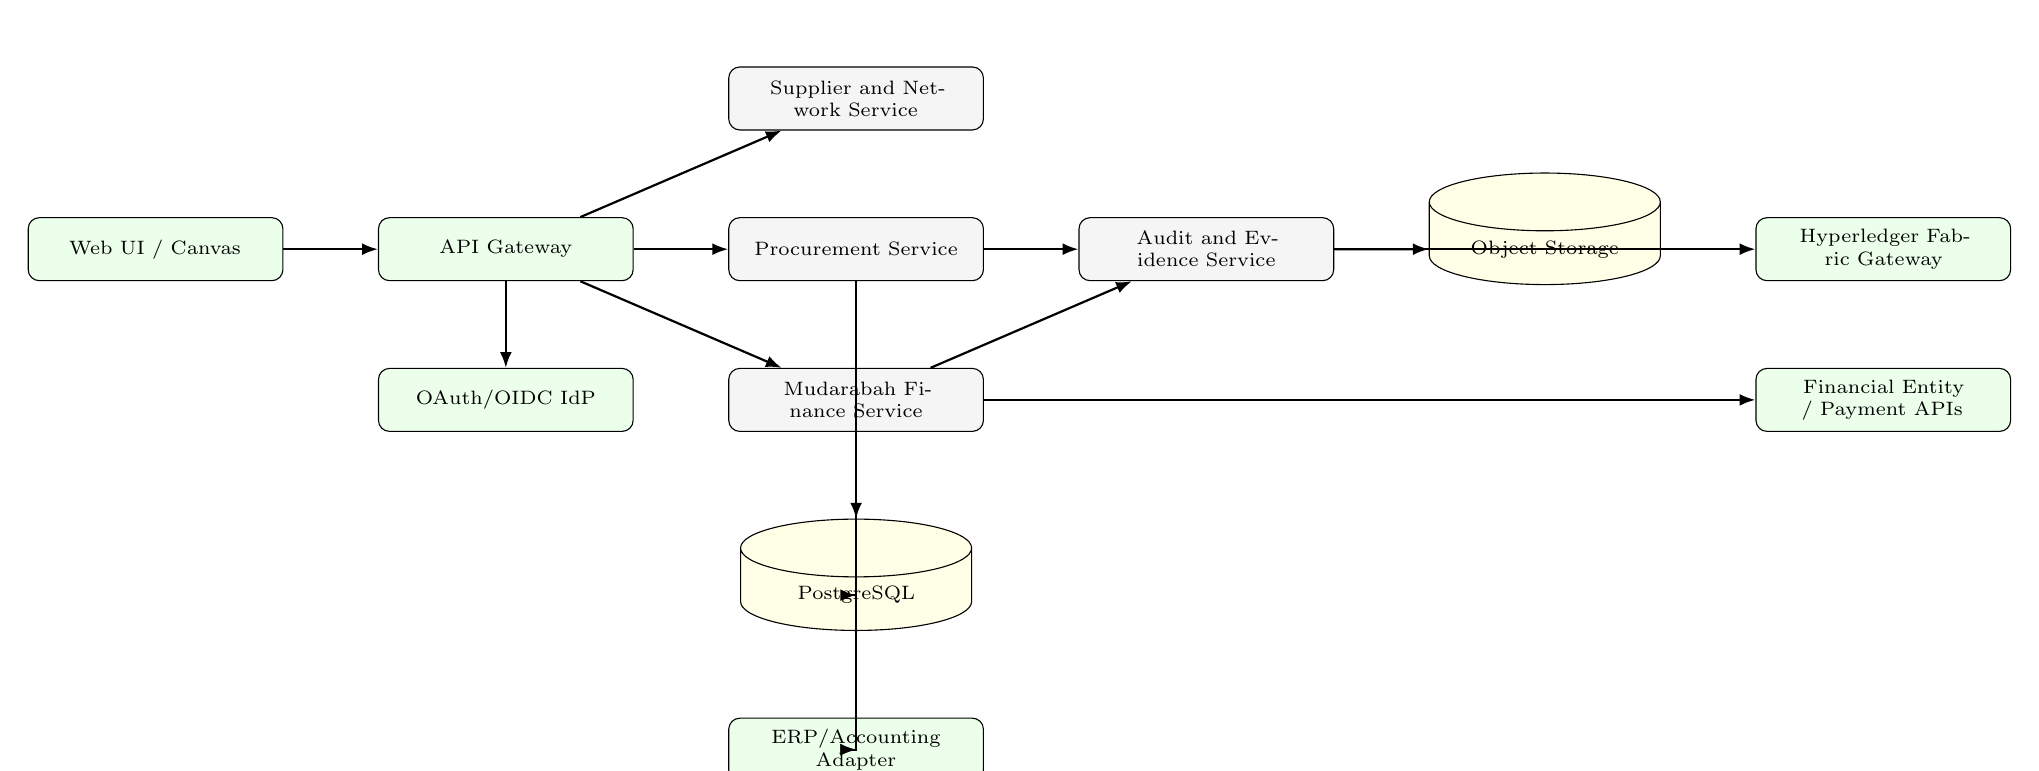
\begin{tikzpicture}[node distance=1.1cm and 1.2cm]
  \node[ext, text width=3.0cm] (web) {Web UI / Canvas};
  \node[ext, right=of web, text width=3.0cm] (api) {API Gateway};
  \node[act, right=of api, text width=3.0cm] (proc) {Procurement Service};
  \node[act, below=of proc, text width=3.0cm] (finance) {Mudarabah Finance Service};
  \node[act, above=of proc, text width=3.0cm] (supplier) {Supplier and Network Service};
  \node[act, right=of proc, text width=3.0cm] (audit) {Audit and Evidence Service};
  \node[datastore, below=of finance, text width=2.7cm] (db) {PostgreSQL};
  \node[datastore, right=of audit, text width=2.7cm] (obj) {Object Storage};
  \node[ext, below=of api, text width=3.0cm] (idp) {OAuth/OIDC IdP};
  \node[ext, below=of db, text width=3.0cm] (erp) {ERP/Accounting Adapter};
  \node[ext, right=of obj, text width=3.0cm] (fabric) {Hyperledger Fabric Gateway};
  \node[ext, below=of fabric, text width=3.0cm] (bank) {Financial Entity / Payment APIs};
  \draw[arrow] (web) -- (api);
  \draw[arrow] (api) -- (proc);
  \draw[arrow] (api) -- (supplier);
  \draw[arrow] (api) -- (finance);
  \draw[arrow] (proc) -- (audit);
  \draw[arrow] (finance) -- (audit);
  \draw[arrow] (audit) -- (obj);
  \draw[arrow] (finance) -- (db);
  \draw[arrow] (proc) |- (db);
  \draw[arrow] (api) -- (idp);
  \draw[arrow] (finance) |- (erp);
  \draw[arrow] (proc) |- (erp);
  \draw[arrow] (audit) -- (fabric);
  \draw[arrow] (finance) -- (bank);
\end{tikzpicture}
\end{adjustbox}
\caption{Logical architecture context for \systemshort{}}
\end{figure}

\subsection{Distributed deployment model}
Each SME deployment is treated as an organization node with its own database, object store, identity configuration, audit log, and integration keys. Cross-organization collaboration uses signed API requests, Fabric event anchors, operator-assisted channel governance, and invitation-based sharing. A financial entity may either install its own node, join as a Fabric organization, or access a hosted financier portal with contractual data segregation.

\subsection{Data confidentiality principle}
The operational database stores full business records. Fabric stores event identifiers, hashes, timestamps, participating organizations, endorsement metadata, and optional private-data references. Unless an explicit sharing rule applies, confidential documents such as invoices, quotations, buyer contracts, and bank details remain off-chain in the owning deployment.
\section{Specific Requirements}

\subsection{Requirement attributes}
Each requirement is assigned an identifier, priority, verification method, and source. Priorities are: P0 mandatory for MVP viability, P1 mandatory for commercial beta, and P2 planned or extensibility requirement. Verification codes may combine inspection, analysis, demonstration, test, and review.
\subsection{Stakeholder needs}\label{sec:stakeholder-needs}
\begin{footnotesize}
\begin{longtable}{@{}p{0.10\textwidth}p{0.10\textwidth}p{0.48\textwidth}p{0.13\textwidth}p{0.13\textwidth}@{}}
\rowcolor{gray!18}\textbf{ID} & \textbf{Priority} & \textbf{Requirement} & \textbf{Verification} & \textbf{Source} \\ \hline
\endfirsthead
\rowcolor{gray!18}\textbf{ID} & \textbf{Priority} & \textbf{Requirement} & \textbf{Verification} & \textbf{Source} \\ \hline
\endhead
\texttt{SN-01} & High & SMEs need to automate procurement workflows without losing control of their own deployment and data. & Review & User vision, procurement thesis \\ \hline
\texttt{SN-02} & High & SME suppliers need access to working capital for confirmed revenue-generating procurement opportunities. & Review & Mudarabah-procurement thesis \\ \hline
\texttt{SN-03} & High & Financial entities need reliable procurement evidence to reduce agency risk and profit-verification cost. & Review & Mudarabah performance report \\ \hline
\texttt{SN-04} & High & Financial entities need controlled monitoring without taking over day-to-day procurement management. & Review & Mudarabah performance report \\ \hline
\texttt{SN-05} & High & Shariah and compliance reviewers need explicit checks for contract form, eligible activity, profit ratio, loss treatment, and breach clauses. & Review & Mudarabah-procurement thesis \\ \hline
\texttt{SN-06} & Medium & Users need a visual supply-chain network view to understand counterparties, dependencies, risks, and financing links. & Demo & User vision \\ \hline
\texttt{SN-07} & High & Organizations need ERP/accounting integration to avoid duplicate records and support reliable project accounting. & Test & Procurement thesis, ERP template \\ \hline
\texttt{SN-08} & High & Auditors need tamper-evident records of key approvals, document versions, financing decisions, and contract lifecycle events. & Inspection & User vision, Fabric design \\ \hline
\texttt{SN-09} & Medium & Administrators need a packaged installation and maintenance workflow suitable for SMEs with limited IT resources. & Demo & User vision, ERP template \\ \hline
\texttt{SN-10} & Medium & Future features need an extension mechanism that does not compromise core procurement, finance, and audit integrity. & Inspection & User vision \\ \hline
\texttt{SN-11} & Medium & Operators and reviewers need health, worker, outbox, Fabric, backup, and deployment evidence without exposing secrets or raw integration payloads. & Demo/Test & Current implementation evidence \\ \hline
\texttt{SN-12} & High & Organizations need Fabric channel governance records that prove proposal, invitation, approval, readiness, and operator execution state without requiring MEPN to hold Fabric admin private keys. & Inspection/Test & Fabric governance decision record \\ \hline
\end{longtable}
\end{footnotesize}
\subsection{Business requirements}\label{sec:business-reqs}
\begin{footnotesize}
\begin{longtable}{@{}p{0.10\textwidth}p{0.10\textwidth}p{0.48\textwidth}p{0.13\textwidth}p{0.13\textwidth}@{}}
\rowcolor{gray!18}\textbf{ID} & \textbf{Priority} & \textbf{Requirement} & \textbf{Verification} & \textbf{Source} \\ \hline
\endfirsthead
\rowcolor{gray!18}\textbf{ID} & \textbf{Priority} & \textbf{Requirement} & \textbf{Verification} & \textbf{Source} \\ \hline
\endhead
\texttt{BR-01} & P0 & The system shall support an end-to-end procurement operating model covering source-to-contract and procure-to-pay activities. & T/D & SN-01 \\ \hline
\texttt{BR-02} & P0 & The system shall support restricted mudarabah financing for procurement opportunities that generate separately measurable revenue or margin. & T/D/R & SN-02,SN-03 \\ \hline
\texttt{BR-03} & P0 & The system shall maintain evidence sufficient to support due diligence, Shariah review, project monitoring, profit/loss calculation, and audit. & I/R & SN-03,SN-05,SN-08 \\ \hline
\texttt{BR-04} & P0 & The system shall prevent a mudarabah application from proceeding to contract execution until required procurement, financial, and Shariah evidence is complete or explicitly waived by authorized reviewers. & T/R & SN-03,SN-05 \\ \hline
\texttt{BR-05} & P1 & The system shall support SME-owned self-hosted deployment and optional managed deployment without changing the functional behavior of procurement and finance workflows. & T/I & SN-01,SN-09 \\ \hline
\texttt{BR-06} & P1 & The system shall permit an SME to invite selected counterparties and financial entities to a bounded opportunity workspace. & T/D & SN-02,SN-03 \\ \hline
\texttt{BR-07} & P1 & The system shall support tamper-evident event anchoring for cross-organization milestones and approvals. & T/I & SN-08 \\ \hline
\texttt{BR-08} & P1 & The system shall provide exportable evidence packs for financier review, Shariah review, dispute handling, and audit. & T/D & SN-03,SN-05,SN-08 \\ \hline
\texttt{BR-09} & P1 & The system shall provide visual supply-chain network visibility for authorized users. & D & SN-06 \\ \hline
\texttt{BR-10} & P2 & The system shall expose extension points for future features through versioned APIs, event subscriptions, and plugin interfaces. & I/T & SN-10 \\ \hline
\texttt{BR-11} & P1 & The system shall provide reviewer-safe operations evidence for health, workers, queues, deployment, backups, reports, and Fabric status without printing or storing secret material. & T/I & SN-09,SN-11 \\ \hline
\texttt{BR-12} & P1 & The system shall support operator-assisted Fabric consortium governance for channel metadata, invitations, approvals, readiness, and sanitized operator evidence. & T/I/R & SN-12 \\ \hline
\end{longtable}
\end{footnotesize}
\subsection{Functional requirements - identity, organization, and administration}\label{sec:fr-identity}
\begin{footnotesize}
\begin{longtable}{@{}p{0.10\textwidth}p{0.10\textwidth}p{0.48\textwidth}p{0.13\textwidth}p{0.13\textwidth}@{}}
\rowcolor{gray!18}\textbf{ID} & \textbf{Priority} & \textbf{Requirement} & \textbf{Verification} & \textbf{Source} \\ \hline
\endfirsthead
\rowcolor{gray!18}\textbf{ID} & \textbf{Priority} & \textbf{Requirement} & \textbf{Verification} & \textbf{Source} \\ \hline
\endhead
\texttt{FR-01} & P0 & The system shall allow an organization administrator to create and maintain organization profile data, including legal name, registration number, tax identifiers, Shariah profile, contact points, profile media such as logo/banner images, and deployment mode. & T/D & BR-05 \\ \hline
\texttt{FR-02} & P0 & The system shall support OAuth 2.0 authorization and OpenID Connect authentication for human users and service clients. & T/I & BR-05 \\ \hline
\texttt{FR-03} & P0 & The system shall enforce role-based access control for organization admin, procurement officer, approver, supplier user, finance user, financier user, Shariah reviewer, auditor, and developer/integrator roles. & T & BR-03 \\ \hline
\texttt{FR-04} & P0 & The system shall permit organization administrators to define approval matrices based on amount, category, project, department, risk level, and financing involvement. & T/D & BR-01 \\ \hline
\texttt{FR-05} & P1 & The system shall record every user login, permission change, organization invitation, and role assignment as an audit event. & T/I & BR-03,BR-07 \\ \hline
\texttt{FR-06} & P1 & The system shall support delegated access for financial entity reviewers limited to the approved opportunity workspace. & T & BR-06 \\ \hline
\texttt{FR-07} & P1 & The system shall provide API client credentials and signed webhook secrets for machine-to-machine integrations. & T/I & BR-10 \\ \hline
\texttt{FR-08} & P2 & The system shall support temporary emergency access grants with justification, expiry time, and mandatory audit review. & T/I & BR-03 \\ \hline
\end{longtable}
\end{footnotesize}
\subsection{Functional requirements - procurement core}\label{sec:fr-procurement}
\begin{footnotesize}
\begin{longtable}{@{}p{0.10\textwidth}p{0.10\textwidth}p{0.48\textwidth}p{0.13\textwidth}p{0.13\textwidth}@{}}
\rowcolor{gray!18}\textbf{ID} & \textbf{Priority} & \textbf{Requirement} & \textbf{Verification} & \textbf{Source} \\ \hline
\endfirsthead
\rowcolor{gray!18}\textbf{ID} & \textbf{Priority} & \textbf{Requirement} & \textbf{Verification} & \textbf{Source} \\ \hline
\endhead
\texttt{FR-09} & P0 & The system shall allow users to create purchase requisitions with item/service specification, quantity, delivery date, budget, department, project, and justification. & T/D & BR-01 \\ \hline
\texttt{FR-10} & P0 & The system shall route purchase requisitions through the configured approval matrix before procurement sourcing or purchase order creation. & T & BR-01 \\ \hline
\texttt{FR-11} & P0 & The system shall allow authorized users to create RFQ, RFP, tender, or direct quotation requests from approved requisitions. & T/D & BR-01 \\ \hline
\texttt{FR-12} & P0 & The system shall allow suppliers to submit quotations with price, delivery schedule, validity date, payment terms, compliance documents, and attachments. & T/D & BR-01 \\ \hline
\texttt{FR-13} & P0 & The system shall provide quotation comparison by price, delivery, supplier score, risk flags, Shariah eligibility, and total expected cost. & T/D & BR-01 \\ \hline
\texttt{FR-14} & P0 & The system shall allow authorized users to create purchase orders from approved quotations, contracts, or direct procurement approvals. & T/D & BR-01 \\ \hline
\texttt{FR-15} & P0 & The system shall track purchase order status from draft through submitted, acknowledged, partially received, received, billed, completed, cancelled, or closed. & T & BR-01 \\ \hline
\texttt{FR-16} & P0 & The system shall allow goods receipts and service confirmations to be recorded against purchase orders with quantity, quality, delivery evidence, and exception notes. & T/D & BR-01 \\ \hline
\texttt{FR-17} & P0 & The system shall allow supplier invoices to be matched against purchase orders and receipts or service confirmations. & T/D & BR-01 \\ \hline
\texttt{FR-18} & P0 & The system shall identify mismatches in quantity, price, tax, delivery, supplier bank details, or duplicate invoice reference before payment approval. & T & BR-01,BR-03 \\ \hline
\texttt{FR-19} & P1 & The system shall maintain supplier onboarding records including registration, bank details, tax data, certifications, Shariah eligibility, risk documents, and approval status. & T/D & BR-01,BR-03 \\ \hline
\texttt{FR-20} & P1 & The system shall calculate supplier performance metrics from delivery timeliness, quality exceptions, invoice exceptions, response rate, and contract compliance. & T/A & BR-01 \\ \hline
\texttt{FR-21} & P1 & The system shall detect potential maverick spending by flagging purchases outside approved suppliers, catalogs, contracts, or approval rules. & T/A & BR-01 \\ \hline
\texttt{FR-22} & P1 & The system shall provide spend analytics by category, supplier, department, project, contract, financing involvement, and time period. & T/D & BR-01 \\ \hline
\texttt{FR-23} & P1 & The system shall allow procurement contracts and framework agreements to be stored with obligations, renewal dates, document versions, and linked POs. & T/D & BR-01 \\ \hline
\texttt{FR-24} & P2 & The system shall support configurable catalog procurement for repeat items and approved supplier price lists. & T/D & BR-01 \\ \hline
\end{longtable}
\end{footnotesize}
\subsection{Functional requirements - mudarabah finance workflow}\label{sec:fr-mudarabah}
\begin{footnotesize}
\begin{longtable}{@{}p{0.10\textwidth}p{0.10\textwidth}p{0.48\textwidth}p{0.13\textwidth}p{0.13\textwidth}@{}}
\rowcolor{gray!18}\textbf{ID} & \textbf{Priority} & \textbf{Requirement} & \textbf{Verification} & \textbf{Source} \\ \hline
\endfirsthead
\rowcolor{gray!18}\textbf{ID} & \textbf{Priority} & \textbf{Requirement} & \textbf{Verification} & \textbf{Source} \\ \hline
\endhead
\texttt{FR-25} & P0 & The system shall allow an authorized SME user to create a procurement opportunity from a buyer PO, contract award, tender result, sales order, or equivalent revenue-generating document. & T/D & BR-02 \\ \hline
\texttt{FR-26} & P0 & The system shall require each mudarabah opportunity to include expected revenue, cost budget, requested capital, delivery timeline, buyer identity, supplier plan, profit-sharing ratio, and risk assumptions. & T/I & BR-02,BR-03 \\ \hline
\texttt{FR-27} & P0 & The system shall prevent a mudarabah application from being submitted if the opportunity is marked as non-revenue-generating or routine internal consumption. & T & BR-02 \\ \hline
\texttt{FR-28} & P0 & The system shall generate a capital application evidence checklist based on opportunity type, sector, amount, buyer risk, supplier risk, and financier policy. & T/D & BR-03 \\ \hline
\texttt{FR-29} & P0 & The system shall provide a due diligence workspace where financial entity users can review buyer credibility, supplier reliability, cost reasonableness, delivery risk, accounting evidence, and repayment/profit realization assumptions. & T/D & BR-03 \\ \hline
\texttt{FR-30} & P0 & The system shall provide a Shariah/compliance review workspace covering eligible goods/services, contract restrictions, profit ratio, guaranteed return prohibition, loss treatment, negligence/breach clauses, and allowed expenses. & T/D/R & BR-03,BR-04 \\ \hline
\texttt{FR-31} & P0 & The system shall require explicit approval or rejection decisions from required financier and Shariah reviewers before contract generation. & T & BR-04 \\ \hline
\texttt{FR-32} & P0 & The system shall generate a restricted mudarabah contract record containing capital amount, project scope, profit ratio, disbursement conditions, reporting duties, permitted expenses, restrictions, loss treatment, breach clauses, dispute process, and signatures. & T/I & BR-02,BR-03 \\ \hline
\texttt{FR-33} & P0 & The system shall support electronic signature workflow or external e-signature integration for contract execution. & T/D & BR-02 \\ \hline
\texttt{FR-34} & P0 & The system shall support disbursement controls including release to controlled account, release to approved supplier, milestone release, and manual release with justification. & T/D & BR-03 \\ \hline
\texttt{FR-35} & P0 & The system shall maintain a project-specific ledger of revenue, capital, procurement costs, allowed expenses, disbursements, buyer payments, profit, loss, and distribution. & T/A & BR-03 \\ \hline
\texttt{FR-36} & P0 & The system shall reconcile project costs against purchase orders, receipts, supplier invoices, payment records, and ERP accounting entries. & T/A & BR-03,BR-08 \\ \hline
\texttt{FR-37} & P0 & The system shall calculate preliminary profit or loss only after required revenue and allowable cost evidence is linked or waived by authorized reviewers. & T/A & BR-03 \\ \hline
\texttt{FR-38} & P0 & The system shall calculate profit distribution according to the approved profit-sharing ratio and shall not calculate a guaranteed fixed return on capital. & T/A/R & BR-02,BR-03 \\ \hline
\texttt{FR-39} & P0 & The system shall route loss cases to an exception workflow that distinguishes genuine commercial loss from negligence, misconduct, fraud, or breach evidence. & T/D/R & BR-03 \\ \hline
\texttt{FR-40} & P1 & The system shall provide financial entity dashboards for application pipeline, exposure, disbursement status, milestone risk, expected realization date, and closure status. & T/D & BR-03 \\ \hline
\texttt{FR-41} & P1 & The system shall allow a financial entity to define policy rules for sectors, maximum exposure, required documents, buyer eligibility, supplier restrictions, and Shariah review thresholds. & T/D & BR-03 \\ \hline
\texttt{FR-42} & P1 & The system shall export a mudarabah closure pack containing contract, approvals, procurement evidence, ledger, profit/loss calculation, distribution record, exceptions, and Fabric anchors. & T/I & BR-08 \\ \hline
\end{longtable}
\end{footnotesize}
\subsection{Functional requirements - network visibility, audit, and extension}\label{sec:fr-network}
\begin{footnotesize}
\begin{longtable}{@{}p{0.10\textwidth}p{0.10\textwidth}p{0.48\textwidth}p{0.13\textwidth}p{0.13\textwidth}@{}}
\rowcolor{gray!18}\textbf{ID} & \textbf{Priority} & \textbf{Requirement} & \textbf{Verification} & \textbf{Source} \\ \hline
\endfirsthead
\rowcolor{gray!18}\textbf{ID} & \textbf{Priority} & \textbf{Requirement} & \textbf{Verification} & \textbf{Source} \\ \hline
\endhead
\texttt{FR-43} & P0 & The system shall represent organizations, suppliers, buyers, financial entities, opportunities, contracts, documents, and financing links as a graph model. & T/I & BR-09 \\ \hline
\texttt{FR-44} & P1 & The system shall provide an interactive canvas where authorized users can add, move, group, filter, and annotate network nodes and edges. & T/D & BR-09 \\ \hline
\texttt{FR-45} & P1 & The system shall color or mark network nodes by status, risk, role, opportunity phase, financing phase, or document completeness. & D & BR-09 \\ \hline
\texttt{FR-46} & P1 & The system shall enforce access control on graph nodes and edges so that users see only relationships and metadata they are authorized to view. & T & BR-03,BR-09 \\ \hline
\texttt{FR-47} & P0 & The system shall create audit events for material cross-organization actions including invitations, RFQ publication, quotation submission, PO acknowledgement, receipt confirmation, invoice submission, financing decision, contract execution, disbursement, profit calculation, and closure. & T/I & BR-07 \\ \hline
\texttt{FR-48} & P0 & The system shall anchor selected audit events to Hyperledger Fabric by writing event hashes, organization identifiers, timestamps, and transaction references to approved channel chaincode. & T/I & BR-07 \\ \hline
\texttt{FR-49} & P1 & The system shall queue Fabric anchoring events when the Fabric gateway is unavailable and retry with idempotency keys. & T & BR-07 \\ \hline
\texttt{FR-50} & P1 & The system shall allow authorized users to verify a document or event against its stored hash and Fabric transaction reference. & T/D & BR-07,BR-08 \\ \hline
\texttt{FR-51} & P1 & The system shall provide organization invitation and membership workflow for adding counterparties to a procurement workspace or network channel. & T/D & BR-06,BR-07 \\ \hline
\texttt{FR-52} & P2 & The system shall provide an extension registry for future modules and shall isolate extensions from core procurement, finance, and audit tables unless explicit permissions are granted. & I/T & BR-10 \\ \hline
\texttt{FR-53} & P1 & The system shall verify real Fabric proof only after querying approved chaincode and comparing the on-chain anchor hash with the local canonical hash and stored audit-anchor hash. & T/I & BR-07,BR-08 \\ \hline
\texttt{FR-54} & P1 & The system shall distinguish mock, pending, anchored, verified, failed, unavailable, and mismatched Fabric evidence states in API and reviewer-facing UI. & T/D & BR-07,BR-08 \\ \hline
\texttt{FR-55} & P1 & The system shall provide operator-assisted Fabric governance for network/channel metadata, invitations, proposal approvals, readiness checks, execution records, and sanitized evidence. & T/I/R & BR-12 \\ \hline
\texttt{FR-56} & P1 & The system shall record operations timeline events for worker heartbeat, outbox, reconciliation, Fabric anchors, report exports, backup/restore, and deployment evidence using sanitized summaries only. & T/I & BR-11 \\ \hline
\end{longtable}
\end{footnotesize}
\subsection{External interface requirements}\label{sec:interfaces}
\begin{footnotesize}
\begin{longtable}{@{}p{0.10\textwidth}p{0.10\textwidth}p{0.48\textwidth}p{0.13\textwidth}p{0.13\textwidth}@{}}
\rowcolor{gray!18}\textbf{ID} & \textbf{Priority} & \textbf{Requirement} & \textbf{Verification} & \textbf{Source} \\ \hline
\endfirsthead
\rowcolor{gray!18}\textbf{ID} & \textbf{Priority} & \textbf{Requirement} & \textbf{Verification} & \textbf{Source} \\ \hline
\endhead
\texttt{IR-01} & P0 & The system shall expose versioned REST APIs documented through OpenAPI for procurement, supplier, financing, audit, graph, and integration functions. & I/T & BR-10 \\ \hline
\texttt{IR-02} & P0 & The system shall support OAuth 2.0 authorization code with PKCE for browser-based user login when integrated with an external identity provider. & T/I & FR-02 \\ \hline
\texttt{IR-03} & P0 & The system shall validate ID token issuer, audience, expiry, signature, and nonce when OpenID Connect is used for authentication. & T/I & FR-02 \\ \hline
\texttt{IR-04} & P0 & The system shall support client credentials flow or signed JWT client authentication for trusted service integrations. & T/I & FR-07 \\ \hline
\texttt{IR-05} & P0 & The system shall support ERP synchronization for suppliers, items, purchase orders, receipts, invoices, payments, chart of accounts, and project ledger entries. & T/D & SN-07 \\ \hline
\texttt{IR-06} & P0 & The ERP adapter shall support idempotent create/update operations using external reference identifiers and reconciliation status. & T & SN-07 \\ \hline
\texttt{IR-07} & P1 & The system shall support CSV/XLSX import and export for SMEs that do not initially expose ERP APIs. & T/D & SN-07 \\ \hline
\texttt{IR-08} & P0 & The Fabric adapter shall connect to an approved gateway endpoint using organization identity material and channel configuration. & T/I & FR-48 \\ \hline
\texttt{IR-09} & P0 & The Fabric adapter shall submit transaction proposals to the configured chaincode and record resulting transaction IDs, block references, and endorsement status. & T/I & FR-48 \\ \hline
\texttt{IR-10} & P1 & The system shall support financial entity API integration for application submission, status retrieval, disbursement instruction, and payment confirmation where the financial entity provides APIs. & T/D & FR-29,FR-34 \\ \hline
\texttt{IR-11} & P1 & The system shall support external e-signature providers through a signed document package, callback validation, and final signed artifact storage. & T/D & FR-33 \\ \hline
\texttt{IR-12} & P1 & The system shall provide webhook subscriptions for procurement milestones, financing decisions, disbursement status, and audit events. & T/I & BR-10 \\ \hline
\texttt{IR-13} & P1 & The system shall expose Fabric governance APIs for networks, channels, memberships, invitations, proposals, approvals, readiness checks, operator execution records, and sanitized evidence retrieval. & T/I & FR-55 \\ \hline
\end{longtable}
\end{footnotesize}
\subsection{Logical data requirements}\label{sec:data}
\begin{footnotesize}
\begin{longtable}{@{}p{0.10\textwidth}p{0.10\textwidth}p{0.48\textwidth}p{0.13\textwidth}p{0.13\textwidth}@{}}
\rowcolor{gray!18}\textbf{ID} & \textbf{Priority} & \textbf{Requirement} & \textbf{Verification} & \textbf{Source} \\ \hline
\endfirsthead
\rowcolor{gray!18}\textbf{ID} & \textbf{Priority} & \textbf{Requirement} & \textbf{Verification} & \textbf{Source} \\ \hline
\endhead
\texttt{DR-01} & P0 & The logical data model shall include Organization, User, Role, Supplier, Buyer, Item, Project, ProcurementOpportunity, Requisition, RFQ, Quotation, PurchaseOrder, Receipt, Invoice, PaymentRecord, and AuditEvent. & I & BR-01 \\ \hline
\texttt{DR-02} & P0 & The logical data model shall include MudarabahApplication, DueDiligenceReport, ShariahReview, MudarabahContract, Disbursement, ProjectLedgerEntry, ProfitLossStatement, ProfitDistribution, and LossException. & I & BR-02,BR-03 \\ \hline
\texttt{DR-03} & P0 & Every material business object shall have organization ownership, lifecycle status, version, created/modified metadata, and audit correlation identifier. & I/T & BR-03 \\ \hline
\texttt{DR-04} & P0 & The system shall maintain immutable document versions after submission, approval, contract execution, or audit anchoring. & T/I & BR-03,BR-07 \\ \hline
\texttt{DR-05} & P0 & The system shall store only cryptographic hashes and minimum required metadata on Fabric unless private data collection rules explicitly permit additional data. & I/T & BR-07 \\ \hline
\texttt{DR-06} & P1 & The system shall support configurable retention policies by document type, organization, contract status, legal hold, and audit requirement. & T/I & BR-03 \\ \hline
\texttt{DR-07} & P1 & The system shall maintain a data lineage link from profit/loss calculations to source procurement documents, ERP postings, and reviewer decisions. & T/I & FR-35,FR-36 \\ \hline
\texttt{DR-08} & P1 & The system shall support master-data validation for supplier identity, bank account, tax details, item categories, units of measure, and organization identifiers. & T & FR-19 \\ \hline
\texttt{DR-09} & P1 & The system shall support anonymized or aggregated analytics exports that exclude confidential document payloads by default. & T/I & BR-09 \\ \hline
\texttt{DR-10} & P2 & The data model shall support custom attributes by organization without requiring core schema modification for common extension fields. & I/T & BR-10 \\ \hline
\texttt{DR-11} & P1 & The logical data model shall include WorkerHeartbeat, IntegrationReconciliationRecord, ReportExportJob, GraphSavedView, GraphAnnotation, and operations timeline read-model support where implemented. & I/T & BR-09,BR-11 \\ \hline
\texttt{DR-12} & P1 & The logical data model shall include FabricNetwork, FabricChannel, FabricChannelMembership, FabricChannelInvitation, FabricChannelProposal, FabricGovernanceApproval, and FabricGovernanceEvidence for operator-assisted governance. & I/T & BR-12 \\ \hline
\end{longtable}
\end{footnotesize}
\subsection{Software system attributes and non-functional requirements}\label{sec:nfr}
\begin{footnotesize}
\begin{longtable}{@{}p{0.09\textwidth}p{0.08\textwidth}p{0.50\textwidth}p{0.16\textwidth}p{0.11\textwidth}@{}}
\rowcolor{gray!18}\textbf{ID} & \textbf{Priority} & \textbf{Requirement} & \textbf{Verification} & \textbf{Source} \\ \hline
\endfirsthead
\rowcolor{gray!18}\textbf{ID} & \textbf{Priority} & \textbf{Requirement} & \textbf{Verification} & \textbf{Source} \\ \hline
\endhead
\texttt{NFR-01} & P0 & The system shall respond to 95 percent of interactive page requests within 2 seconds under the agreed SME reference load excluding external system latency. & Performance test & BR-01 \\ \hline
\texttt{NFR-02} & P0 & The system shall process 95 percent of standard procurement workflow transitions within 1 second after request validation excluding external integrations. & Performance test & BR-01 \\ \hline
\texttt{NFR-03} & P1 & The system shall support at least 100 concurrent users per SME deployment on the reference hardware profile defined in the deployment guide. & Load test & BR-05 \\ \hline
\texttt{NFR-04} & P1 & The system shall support at least 100,000 procurement documents per organization without functional degradation when indexed and archived according to guidance. & Load test & BR-05 \\ \hline
\texttt{NFR-05} & P0 & The system shall encrypt traffic using TLS 1.2 or higher for all browser, API, ERP adapter, financial entity, and Fabric gateway connections. & Security test & FR-02,IR-08 \\ \hline
\texttt{NFR-06} & P0 & The system shall encrypt secrets at rest using a managed secrets store or deployment-approved equivalent, and mounted secret files shall not be printed, logged, committed, or exposed in screenshots/evidence. & Inspection & FR-07 \\ \hline
\texttt{NFR-07} & P0 & The system shall enforce tenant and organization data isolation at the application service and database access layers. & Security test & BR-05 \\ \hline
\texttt{NFR-08} & P0 & The system shall reject access tokens that are expired, issued by an untrusted issuer, signed by an untrusted key, or missing required audience/scope claims. & Security test & FR-02 \\ \hline
\texttt{NFR-09} & P0 & The system shall maintain an append-only audit log for authentication, authorization, workflow, data change, document, integration, and Fabric anchoring events. & Inspection/Test & BR-03,BR-07 \\ \hline
\texttt{NFR-10} & P1 & The system shall provide backup and restore procedures with a recovery point objective of 24 hours and a recovery time objective of 8 hours for SME self-hosted deployments. & DR test & BR-05 \\ \hline
\texttt{NFR-11} & P1 & The system shall queue outbound ERP, Fabric, e-signature, and financial entity events and retry them without duplicate business effects. & Integration test & IR-06,IR-09,IR-10 \\ \hline
\texttt{NFR-12} & P1 & The system shall continue core local procurement operations when Fabric is unavailable, with clear user indication that anchors are pending. & Resilience test & FR-49 \\ \hline
\texttt{NFR-13} & P1 & The system shall provide observable logs, metrics, traces, and health checks for application, database, queue, adapter, and Fabric connectivity components. & Inspection/Test & BR-05 \\ \hline
\texttt{NFR-14} & P1 & The system shall support configurable localization for currency, date format, tax labels, document numbering, and language packs. & Demo & BR-05 \\ \hline
\texttt{NFR-15} & P1 & The system shall meet WCAG 2.1 AA principles for core procurement and finance workflows where technically feasible. & Accessibility review & User characteristics \\ \hline
\texttt{NFR-16} & P1 & The system shall provide clear validation messages for missing financing evidence, Shariah checklist failures, and procurement matching exceptions. & Usability test & BR-03,BR-04 \\ \hline
\texttt{NFR-17} & P0 & The system shall prevent modification of executed contract terms except through a versioned amendment workflow. & Security/Workflow test & FR-32 \\ \hline
\texttt{NFR-18} & P0 & The system shall not store full supplier bank account details in Fabric event payloads. & Inspection/Test & DR-05 \\ \hline
\texttt{NFR-19} & P1 & The system shall support deployment through Docker Compose with documented environment variables, secrets, migration, backup, and upgrade steps. & Installation test & BR-05 \\ \hline
\texttt{NFR-20} & P2 & The system should support Kubernetes deployment through Helm charts for financial entities or managed consortium operators. & Installation test & BR-05 \\ \hline
\texttt{NFR-21} & P1 & The system shall allow administrators to configure data residency boundaries for storage, backups, and Fabric channel participation. & Inspection/Demo & BR-05 \\ \hline
\texttt{NFR-22} & P1 & The system shall provide vulnerability scanning and dependency report generation as part of the release pipeline. & Inspection & Security \\ \hline
\texttt{NFR-23} & P1 & The system shall support evidence/report export in machine-readable JSON and CSV package formats for the FYP baseline, with PDF/spreadsheet report packs tracked as production hardening until implemented. & Test/Demo & BR-08 \\ \hline
\texttt{NFR-24} & P2 & The system should support plugin sandboxing to limit future extension access to explicit API scopes. & Security review & BR-10 \\ \hline
\end{longtable}
\end{footnotesize}
\subsection{Verification method definitions}
\begin{footnotesize}
\begin{longtable}{@{}p{0.20\textwidth}p{0.75\textwidth}@{}}
\rowcolor{gray!18}\textbf{Method} & \textbf{Definition} \\ \hline
\endfirsthead
\rowcolor{gray!18}\textbf{Method} & \textbf{Definition} \\ \hline
\endhead
Inspection & Examination of documents, configuration, code, schema, logs, or deployed settings. \\ \hline
Analysis & Reasoned evaluation, calculation, model review, threat modeling, or consistency checking. \\ \hline
Demonstration & Observed execution of a workflow using representative data without deep instrumentation. \\ \hline
Test & Repeatable procedure with expected input, output, assertions, and pass/fail criteria. \\ \hline
Review & Stakeholder, Shariah, legal, accounting, compliance, or operational acceptance review. \\ \hline
\end{longtable}
\end{footnotesize}
\section{UML Requirements Model}



\begin{landscape}
\subsection{Use Case Diagram}
\begin{figure}[h!]
\centering
\begin{adjustbox}{max width=1.05\linewidth}
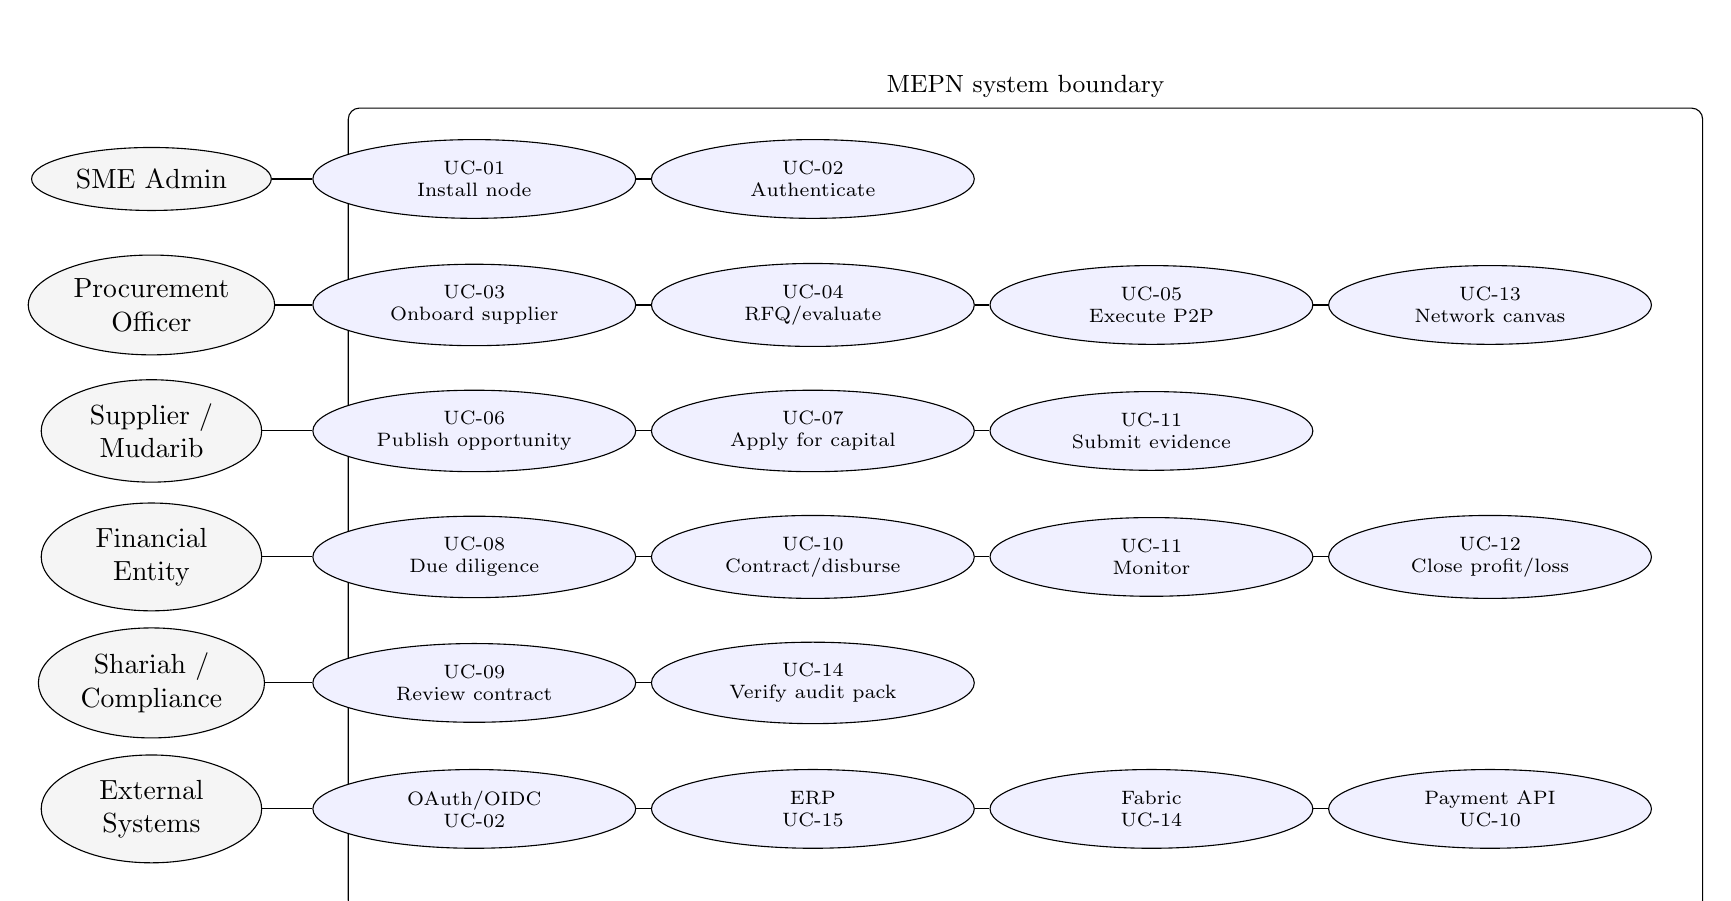
\begin{tikzpicture}[x=1cm,y=1cm]
  \node[draw, rounded corners, minimum width=17.2cm, minimum height=10.2cm, label={[font=\small]above:MEPN system boundary}] (boundary) at (1.3,0.3) {};

  \node[actor] (admin) at (-9.8,4.5) {SME Admin};
  \node[usecasebig] (a1) at (-5.7,4.5) {UC-01\\Install node};
  \node[usecasebig] (a2) at (-1.4,4.5) {UC-02\\Authenticate};
  \draw (admin.east) -- (a1.west); \draw (a1.east) -- (a2.west);

  \node[actor] (proc) at (-9.8,2.9) {Procurement\\Officer};
  \node[usecasebig] (p1) at (-5.7,2.9) {UC-03\\Onboard supplier};
  \node[usecasebig] (p2) at (-1.4,2.9) {UC-04\\RFQ/evaluate};
  \node[usecasebig] (p3) at (2.9,2.9) {UC-05\\Execute P2P};
  \node[usecasebig] (p4) at (7.2,2.9) {UC-13\\Network canvas};
  \draw (proc.east) -- (p1.west); \draw (p1.east) -- (p2.west); \draw (p2.east) -- (p3.west); \draw (p3.east) -- (p4.west);

  \node[actor] (sup) at (-9.8,1.3) {Supplier /\\Mudarib};
  \node[usecasebig] (s1) at (-5.7,1.3) {UC-06\\Publish opportunity};
  \node[usecasebig] (s2) at (-1.4,1.3) {UC-07\\Apply for capital};
  \node[usecasebig] (s3) at (2.9,1.3) {UC-11\\Submit evidence};
  \draw (sup.east) -- (s1.west); \draw (s1.east) -- (s2.west); \draw (s2.east) -- (s3.west);

  \node[actor] (fe) at (-9.8,-0.3) {Financial\\Entity};
  \node[usecasebig] (f1) at (-5.7,-0.3) {UC-08\\Due diligence};
  \node[usecasebig] (f2) at (-1.4,-0.3) {UC-10\\Contract/disburse};
  \node[usecasebig] (f3) at (2.9,-0.3) {UC-11\\Monitor};
  \node[usecasebig] (f4) at (7.2,-0.3) {UC-12\\Close profit/loss};
  \draw (fe.east) -- (f1.west); \draw (f1.east) -- (f2.west); \draw (f2.east) -- (f3.west); \draw (f3.east) -- (f4.west);

  \node[actor] (sha) at (-9.8,-1.9) {Shariah /\\Compliance};
  \node[usecasebig] (sh1) at (-5.7,-1.9) {UC-09\\Review contract};
  \node[usecasebig] (sh2) at (-1.4,-1.9) {UC-14\\Verify audit pack};
  \draw (sha.east) -- (sh1.west); \draw (sh1.east) -- (sh2.west);

  \node[actor] (int) at (-9.8,-3.5) {External\\Systems};
  \node[usecasebig] (i1) at (-5.7,-3.5) {OAuth/OIDC\\UC-02};
  \node[usecasebig] (i2) at (-1.4,-3.5) {ERP\\UC-15};
  \node[usecasebig] (i3) at (2.9,-3.5) {Fabric\\UC-14};
  \node[usecasebig] (i4) at (7.2,-3.5) {Payment API\\UC-10};
  \draw (int.east) -- (i1.west); \draw (i1.east) -- (i2.west); \draw (i2.east) -- (i3.west); \draw (i3.east) -- (i4.west);
\end{tikzpicture}
\end{adjustbox}
\caption{Use case diagram for \systemshort{} showing actor-oriented use case groups}
\end{figure}
\end{landscape}

\subsection{Use Case Specifications}
\subsubsection{UC-01 - Install and configure SME node}
\begin{footnotesize}
\begin{longtable}{@{}p{0.22\textwidth}p{0.72\textwidth}@{}}
\rowcolor{gray!10}\textbf{Use case ID and name} & UC-01 - Install and configure SME node \\ \hline
\rowcolor{gray!10}\textbf{Primary actor} & SME Owner/Admin \\ \hline
\rowcolor{gray!10}\textbf{Supporting actors} & Developer/Integrator, Identity Provider, ERP system \\ \hline
\rowcolor{gray!10}\textbf{Goal} & Deploy a functioning self-hosted or managed organization node. \\ \hline
\rowcolor{gray!10}\textbf{Preconditions} & Installation package is available; administrator has infrastructure and organization details. \\ \hline
\rowcolor{gray!10}\textbf{Trigger} & Administrator starts first-run setup. \\ \hline
\rowcolor{gray!10}\textbf{Main success scenario} & 1. Launch deployment. 2. Create organization profile. 3. Configure identity provider. 4. Configure database, object storage, email, and queue. 5. Create administrator role. 6. Run health checks. 7. Enable backup schedule. \\ \hline
\rowcolor{gray!10}\textbf{Alternate or exception flows} & A1: Identity provider unavailable - administrator uses local bootstrap admin and completes IdP configuration later. A2: ERP not ready - node operates without ERP adapter. \\ \hline
\rowcolor{gray!10}\textbf{Postconditions} & Organization node is operational, audited, and ready for procurement setup. \\ \hline
\rowcolor{gray!10}\textbf{Related requirements} & FR-01, FR-02, FR-03, NFR-10, NFR-19 \\ \hline
\end{longtable}
\end{footnotesize}
\subsubsection{UC-02 - Authenticate and authorize user}
\begin{footnotesize}
\begin{longtable}{@{}p{0.22\textwidth}p{0.72\textwidth}@{}}
\rowcolor{gray!10}\textbf{Use case ID and name} & UC-02 - Authenticate and authorize user \\ \hline
\rowcolor{gray!10}\textbf{Primary actor} & Any human user \\ \hline
\rowcolor{gray!10}\textbf{Supporting actors} & OAuth/OIDC identity provider, API gateway \\ \hline
\rowcolor{gray!10}\textbf{Goal} & Access authorized system functions with correct organization context. \\ \hline
\rowcolor{gray!10}\textbf{Preconditions} & User exists in IdP or local invite workflow; organization role exists. \\ \hline
\rowcolor{gray!10}\textbf{Trigger} & User opens the web application. \\ \hline
\rowcolor{gray!10}\textbf{Main success scenario} & 1. User starts login. 2. System redirects to IdP. 3. User authenticates. 4. System validates tokens. 5. System maps claims to organization roles. 6. Authorized landing page is shown. \\ \hline
\rowcolor{gray!10}\textbf{Alternate or exception flows} & A1: Invalid token - request is rejected. A2: Missing role - user sees no-access page and audit event is created. \\ \hline
\rowcolor{gray!10}\textbf{Postconditions} & Session is established with role-scoped permissions or access is denied. \\ \hline
\rowcolor{gray!10}\textbf{Related requirements} & FR-02, FR-03, FR-05, IR-02, IR-03, NFR-08 \\ \hline
\end{longtable}
\end{footnotesize}
\subsubsection{UC-03 - Onboard supplier}
\begin{footnotesize}
\begin{longtable}{@{}p{0.22\textwidth}p{0.72\textwidth}@{}}
\rowcolor{gray!10}\textbf{Use case ID and name} & UC-03 - Onboard supplier \\ \hline
\rowcolor{gray!10}\textbf{Primary actor} & Procurement Officer \\ \hline
\rowcolor{gray!10}\textbf{Supporting actors} & Supplier User, Finance/Accountant, Shariah Reviewer \\ \hline
\rowcolor{gray!10}\textbf{Goal} & Create an approved supplier record with risk and compliance evidence. \\ \hline
\rowcolor{gray!10}\textbf{Preconditions} & Procurement officer has supplier management rights. \\ \hline
\rowcolor{gray!10}\textbf{Trigger} & A new supplier is required or a supplier responds to an invitation. \\ \hline
\rowcolor{gray!10}\textbf{Main success scenario} & 1. Create supplier profile. 2. Request documents. 3. Supplier submits registration, bank, tax, certification, and Shariah information. 4. System validates completeness. 5. Reviewer approves, rejects, or requests changes. 6. Supplier becomes available for sourcing. \\ \hline
\rowcolor{gray!10}\textbf{Alternate or exception flows} & A1: Bank details mismatch - supplier is blocked for payment use. A2: Shariah eligibility unresolved - supplier can be marked restricted. \\ \hline
\rowcolor{gray!10}\textbf{Postconditions} & Supplier has status, evidence, and approval history. \\ \hline
\rowcolor{gray!10}\textbf{Related requirements} & FR-19, FR-20, DR-08, NFR-16 \\ \hline
\end{longtable}
\end{footnotesize}
\subsubsection{UC-04 - Run RFQ and supplier evaluation}
\begin{footnotesize}
\begin{longtable}{@{}p{0.22\textwidth}p{0.72\textwidth}@{}}
\rowcolor{gray!10}\textbf{Use case ID and name} & UC-04 - Run RFQ and supplier evaluation \\ \hline
\rowcolor{gray!10}\textbf{Primary actor} & Procurement Officer \\ \hline
\rowcolor{gray!10}\textbf{Supporting actors} & Supplier User, Approver/Manager \\ \hline
\rowcolor{gray!10}\textbf{Goal} & Select a supplier through controlled sourcing. \\ \hline
\rowcolor{gray!10}\textbf{Preconditions} & Approved requisition or sourcing need exists. \\ \hline
\rowcolor{gray!10}\textbf{Trigger} & Procurement officer creates RFQ/RFP/tender. \\ \hline
\rowcolor{gray!10}\textbf{Main success scenario} & 1. Create RFQ from requirement. 2. Invite suppliers. 3. Suppliers submit quotations. 4. System compares quotations. 5. Procurement officer recommends award. 6. Approver approves. 7. Award record is stored. \\ \hline
\rowcolor{gray!10}\textbf{Alternate or exception flows} & A1: Supplier misses deadline - quotation is excluded unless authorized exception. A2: Conflict of interest flag - additional approval required. \\ \hline
\rowcolor{gray!10}\textbf{Postconditions} & Approved supplier quotation or award exists for PO creation and optional financing evidence. \\ \hline
\rowcolor{gray!10}\textbf{Related requirements} & FR-11, FR-12, FR-13, FR-23 \\ \hline
\end{longtable}
\end{footnotesize}
\subsubsection{UC-05 - Execute procure-to-pay workflow}
\begin{footnotesize}
\begin{longtable}{@{}p{0.22\textwidth}p{0.72\textwidth}@{}}
\rowcolor{gray!10}\textbf{Use case ID and name} & UC-05 - Execute procure-to-pay workflow \\ \hline
\rowcolor{gray!10}\textbf{Primary actor} & Procurement Officer \\ \hline
\rowcolor{gray!10}\textbf{Supporting actors} & Approver/Manager, Supplier User, Finance/Accountant, ERP system \\ \hline
\rowcolor{gray!10}\textbf{Goal} & Create and close a purchase transaction with matching evidence. \\ \hline
\rowcolor{gray!10}\textbf{Preconditions} & Approved requisition or quotation exists; supplier is approved. \\ \hline
\rowcolor{gray!10}\textbf{Trigger} & Purchase order is created. \\ \hline
\rowcolor{gray!10}\textbf{Main success scenario} & 1. Generate PO. 2. Route for approval. 3. Supplier acknowledges. 4. Goods or services are received. 5. Supplier submits invoice. 6. System performs three-way match. 7. Finance approves payment status or ERP posting. 8. PO is completed or closed. \\ \hline
\rowcolor{gray!10}\textbf{Alternate or exception flows} & A1: Match exception - invoice enters exception workflow. A2: Partial delivery - PO remains partially received. A3: Supplier on hold - PO submission blocked. \\ \hline
\rowcolor{gray!10}\textbf{Postconditions} & Procurement transaction has auditable document chain and ERP reconciliation status. \\ \hline
\rowcolor{gray!10}\textbf{Related requirements} & FR-09 to FR-18, IR-05, IR-06 \\ \hline
\end{longtable}
\end{footnotesize}
\subsubsection{UC-06 - Publish procurement opportunity for financing}
\begin{footnotesize}
\begin{longtable}{@{}p{0.22\textwidth}p{0.72\textwidth}@{}}
\rowcolor{gray!10}\textbf{Use case ID and name} & UC-06 - Publish procurement opportunity for financing \\ \hline
\rowcolor{gray!10}\textbf{Primary actor} & SME Supplier/Mudarib \\ \hline
\rowcolor{gray!10}\textbf{Supporting actors} & Buyer, Procurement Officer, Finance/Accountant \\ \hline
\rowcolor{gray!10}\textbf{Goal} & Create a revenue-generating procurement opportunity that can be financed. \\ \hline
\rowcolor{gray!10}\textbf{Preconditions} & Buyer PO, sales order, tender award, or contract evidence exists. \\ \hline
\rowcolor{gray!10}\textbf{Trigger} & Mudarib needs capital to execute the opportunity. \\ \hline
\rowcolor{gray!10}\textbf{Main success scenario} & 1. Create opportunity record. 2. Attach buyer demand evidence. 3. Add expected revenue, supplier plan, cost budget, delivery timeline, risk assumptions, and requested capital. 4. System checks suitability. 5. Opportunity is submitted for financing. \\ \hline
\rowcolor{gray!10}\textbf{Alternate or exception flows} & A1: Opportunity is internal consumption - system blocks mudarabah submission. A2: Evidence missing - application remains draft. \\ \hline
\rowcolor{gray!10}\textbf{Postconditions} & Opportunity is ready for financier invitation or internal review. \\ \hline
\rowcolor{gray!10}\textbf{Related requirements} & FR-25, FR-26, FR-27, FR-28 \\ \hline
\end{longtable}
\end{footnotesize}
\subsubsection{UC-07 - Apply for mudarabah capital}
\begin{footnotesize}
\begin{longtable}{@{}p{0.22\textwidth}p{0.72\textwidth}@{}}
\rowcolor{gray!10}\textbf{Use case ID and name} & UC-07 - Apply for mudarabah capital \\ \hline
\rowcolor{gray!10}\textbf{Primary actor} & SME Supplier/Mudarib \\ \hline
\rowcolor{gray!10}\textbf{Supporting actors} & Financial Entity User, Shariah Reviewer \\ \hline
\rowcolor{gray!10}\textbf{Goal} & Submit a complete capital application for restricted mudarabah financing. \\ \hline
\rowcolor{gray!10}\textbf{Preconditions} & Procurement opportunity exists and passes suitability checks. \\ \hline
\rowcolor{gray!10}\textbf{Trigger} & Mudarib sends application to a financial entity. \\ \hline
\rowcolor{gray!10}\textbf{Main success scenario} & 1. Select financier. 2. Confirm requested capital and profit ratio proposal. 3. Submit evidence checklist. 4. System creates restricted workspace. 5. Financial entity receives application notification. \\ \hline
\rowcolor{gray!10}\textbf{Alternate or exception flows} & A1: Financier policy requires extra documents - system requests additional evidence. A2: Profit ratio omitted - submission blocked. \\ \hline
\rowcolor{gray!10}\textbf{Postconditions} & Application is in submitted state with audit record and workspace access. \\ \hline
\rowcolor{gray!10}\textbf{Related requirements} & FR-26, FR-28, FR-29, FR-41 \\ \hline
\end{longtable}
\end{footnotesize}
\subsubsection{UC-08 - Perform financier due diligence}
\begin{footnotesize}
\begin{longtable}{@{}p{0.22\textwidth}p{0.72\textwidth}@{}}
\rowcolor{gray!10}\textbf{Use case ID and name} & UC-08 - Perform financier due diligence \\ \hline
\rowcolor{gray!10}\textbf{Primary actor} & Financial Entity Investment Officer \\ \hline
\rowcolor{gray!10}\textbf{Supporting actors} & SME Supplier/Mudarib, Buyer, Supplier, ERP system \\ \hline
\rowcolor{gray!10}\textbf{Goal} & Assess commercial viability and risk of the application. \\ \hline
\rowcolor{gray!10}\textbf{Preconditions} & Application is submitted and reviewer has workspace access. \\ \hline
\rowcolor{gray!10}\textbf{Trigger} & Investment officer opens due diligence task. \\ \hline
\rowcolor{gray!10}\textbf{Main success scenario} & 1. Review buyer evidence. 2. Review supplier plan and quotations. 3. Review project economics. 4. Review ERP/accounting history. 5. Record findings and conditions. 6. Approve, reject, or request changes. \\ \hline
\rowcolor{gray!10}\textbf{Alternate or exception flows} & A1: Buyer cannot be verified - application is rejected or paused. A2: Cost budget unreasonable - application returns for revision. \\ \hline
\rowcolor{gray!10}\textbf{Postconditions} & Due diligence decision is recorded with evidence and conditions. \\ \hline
\rowcolor{gray!10}\textbf{Related requirements} & FR-29, FR-41, DR-07 \\ \hline
\end{longtable}
\end{footnotesize}
\subsubsection{UC-09 - Perform Shariah and compliance review}
\begin{footnotesize}
\begin{longtable}{@{}p{0.22\textwidth}p{0.72\textwidth}@{}}
\rowcolor{gray!10}\textbf{Use case ID and name} & UC-09 - Perform Shariah and compliance review \\ \hline
\rowcolor{gray!10}\textbf{Primary actor} & Shariah/Compliance Reviewer \\ \hline
\rowcolor{gray!10}\textbf{Supporting actors} & Financial Entity User, SME Supplier/Mudarib \\ \hline
\rowcolor{gray!10}\textbf{Goal} & Validate contract eligibility and compliance controls. \\ \hline
\rowcolor{gray!10}\textbf{Preconditions} & Application and due diligence evidence are available. \\ \hline
\rowcolor{gray!10}\textbf{Trigger} & Reviewer receives Shariah/compliance review task. \\ \hline
\rowcolor{gray!10}\textbf{Main success scenario} & 1. Review goods/services. 2. Review buyer and supplier restrictions. 3. Review profit ratio. 4. Review loss and negligence clauses. 5. Review allowed expenses. 6. Approve, reject, or request amendments. \\ \hline
\rowcolor{gray!10}\textbf{Alternate or exception flows} & A1: Goods/services not eligible - application rejected. A2: Profit term implies guaranteed fixed return - amendment required. \\ \hline
\rowcolor{gray!10}\textbf{Postconditions} & Compliance decision and checklist are stored. \\ \hline
\rowcolor{gray!10}\textbf{Related requirements} & FR-30, FR-31, FR-32 \\ \hline
\end{longtable}
\end{footnotesize}
\subsubsection{UC-10 - Execute mudarabah contract and disburse capital}
\begin{footnotesize}
\begin{longtable}{@{}p{0.22\textwidth}p{0.72\textwidth}@{}}
\rowcolor{gray!10}\textbf{Use case ID and name} & UC-10 - Execute mudarabah contract and disburse capital \\ \hline
\rowcolor{gray!10}\textbf{Primary actor} & Financial Entity User \\ \hline
\rowcolor{gray!10}\textbf{Supporting actors} & SME Supplier/Mudarib, Shariah Reviewer, E-signature provider, Payment API \\ \hline
\rowcolor{gray!10}\textbf{Goal} & Create binding contract record and release capital under approved controls. \\ \hline
\rowcolor{gray!10}\textbf{Preconditions} & Due diligence and Shariah review are approved. \\ \hline
\rowcolor{gray!10}\textbf{Trigger} & Financial entity initiates contract execution. \\ \hline
\rowcolor{gray!10}\textbf{Main success scenario} & 1. Generate contract from approved terms. 2. Parties review. 3. Parties sign. 4. System locks contract version. 5. Financial entity chooses disbursement method. 6. Disbursement is recorded and optionally sent to payment API. 7. Audit/Fabric event is created. \\ \hline
\rowcolor{gray!10}\textbf{Alternate or exception flows} & A1: Signature rejected - contract returns for correction. A2: Payment API unavailable - disbursement instruction is queued or manually recorded. \\ \hline
\rowcolor{gray!10}\textbf{Postconditions} & Contract is executed and capital release status is recorded. \\ \hline
\rowcolor{gray!10}\textbf{Related requirements} & FR-32, FR-33, FR-34, FR-47, FR-48 \\ \hline
\end{longtable}
\end{footnotesize}
\subsubsection{UC-11 - Monitor procurement execution}
\begin{footnotesize}
\begin{longtable}{@{}p{0.22\textwidth}p{0.72\textwidth}@{}}
\rowcolor{gray!10}\textbf{Use case ID and name} & UC-11 - Monitor procurement execution \\ \hline
\rowcolor{gray!10}\textbf{Primary actor} & Financial Entity User \\ \hline
\rowcolor{gray!10}\textbf{Supporting actors} & SME Supplier/Mudarib, Procurement Officer, Supplier User, Buyer \\ \hline
\rowcolor{gray!10}\textbf{Goal} & Track milestones without interfering with mudarib management. \\ \hline
\rowcolor{gray!10}\textbf{Preconditions} & Contract executed and project ledger active. \\ \hline
\rowcolor{gray!10}\textbf{Trigger} & Procurement execution begins or milestone changes. \\ \hline
\rowcolor{gray!10}\textbf{Main success scenario} & 1. System imports or records POs, receipts, invoices, payments, and exceptions. 2. Dashboard updates milestone and risk status. 3. User reviews variances. 4. Evidence requests are issued if needed. 5. Critical events are anchored. \\ \hline
\rowcolor{gray!10}\textbf{Alternate or exception flows} & A1: Delivery delay - risk flag and notification. A2: Cost overrun - approval or amendment workflow. A3: Missing receipt - profit calculation blocked. \\ \hline
\rowcolor{gray!10}\textbf{Postconditions} & Project status and evidence are current. \\ \hline
\rowcolor{gray!10}\textbf{Related requirements} & FR-35, FR-36, FR-40, FR-47, FR-49 \\ \hline
\end{longtable}
\end{footnotesize}
\subsubsection{UC-12 - Calculate profit/loss and close mudarabah project}
\begin{footnotesize}
\begin{longtable}{@{}p{0.22\textwidth}p{0.72\textwidth}@{}}
\rowcolor{gray!10}\textbf{Use case ID and name} & UC-12 - Calculate profit/loss and close mudarabah project \\ \hline
\rowcolor{gray!10}\textbf{Primary actor} & Finance/Accountant \\ \hline
\rowcolor{gray!10}\textbf{Supporting actors} & Financial Entity User, SME Supplier/Mudarib, Shariah Reviewer, Auditor \\ \hline
\rowcolor{gray!10}\textbf{Goal} & Compute and approve project outcome and distribution. \\ \hline
\rowcolor{gray!10}\textbf{Preconditions} & Revenue, cost, payment, and expense evidence is complete or waived. \\ \hline
\rowcolor{gray!10}\textbf{Trigger} & Buyer payment is received or project closure is requested. \\ \hline
\rowcolor{gray!10}\textbf{Main success scenario} & 1. System compiles project ledger. 2. System calculates allowable costs. 3. System calculates net profit or loss. 4. Reviewers verify calculation. 5. Profit is distributed by approved ratio or loss workflow is started. 6. Closure pack is generated. 7. Contract is closed. \\ \hline
\rowcolor{gray!10}\textbf{Alternate or exception flows} & A1: Loss detected - loss exception workflow determines genuine loss vs breach. A2: Expense disputed - calculation paused pending resolution. \\ \hline
\rowcolor{gray!10}\textbf{Postconditions} & Project is closed with auditable calculation and distribution or loss decision. \\ \hline
\rowcolor{gray!10}\textbf{Related requirements} & FR-35, FR-37, FR-38, FR-39, FR-42 \\ \hline
\end{longtable}
\end{footnotesize}
\subsubsection{UC-13 - Use supply-chain network canvas}
\begin{footnotesize}
\begin{longtable}{@{}p{0.22\textwidth}p{0.72\textwidth}@{}}
\rowcolor{gray!10}\textbf{Use case ID and name} & UC-13 - Use supply-chain network canvas \\ \hline
\rowcolor{gray!10}\textbf{Primary actor} & Procurement Officer or Financial Entity User \\ \hline
\rowcolor{gray!10}\textbf{Supporting actors} & Graph service, audit service \\ \hline
\rowcolor{gray!10}\textbf{Goal} & Visualize relationships, status, risk, and finance dependencies. \\ \hline
\rowcolor{gray!10}\textbf{Preconditions} & User has graph view permission. \\ \hline
\rowcolor{gray!10}\textbf{Trigger} & User opens network canvas. \\ \hline
\rowcolor{gray!10}\textbf{Main success scenario} & 1. System loads authorized graph nodes and edges. 2. User filters by organization, supplier, opportunity, status, risk, or financing phase. 3. User expands node details. 4. User adds comments or annotations. 5. System saves view snapshot. \\ \hline
\rowcolor{gray!10}\textbf{Alternate or exception flows} & A1: User lacks permission - node metadata is redacted. A2: Graph query is large - system prompts filter refinement. \\ \hline
\rowcolor{gray!10}\textbf{Postconditions} & User obtains authorized network visibility without exposing unauthorized data. \\ \hline
\rowcolor{gray!10}\textbf{Related requirements} & FR-43, FR-44, FR-45, FR-46 \\ \hline
\end{longtable}
\end{footnotesize}
\subsubsection{UC-14 - Verify audit event and evidence pack}
\begin{footnotesize}
\begin{longtable}{@{}p{0.22\textwidth}p{0.72\textwidth}@{}}
\rowcolor{gray!10}\textbf{Use case ID and name} & UC-14 - Verify audit event and evidence pack \\ \hline
\rowcolor{gray!10}\textbf{Primary actor} & Auditor \\ \hline
\rowcolor{gray!10}\textbf{Supporting actors} & Fabric Gateway, Audit Service, Object Storage \\ \hline
\rowcolor{gray!10}\textbf{Goal} & Confirm that a document or event matches stored system and Fabric evidence. \\ \hline
\rowcolor{gray!10}\textbf{Preconditions} & Auditor has read-only access to evidence pack. \\ \hline
\rowcolor{gray!10}\textbf{Trigger} & Audit review begins or dispute arises. \\ \hline
\rowcolor{gray!10}\textbf{Main success scenario} & 1. Auditor opens evidence pack. 2. System shows document version, hash, workflow history, user actions, and Fabric transaction reference. 3. Auditor verifies hash. 4. System retrieves Fabric transaction metadata. 5. Auditor records finding. \\ \hline
\rowcolor{gray!10}\textbf{Alternate or exception flows} & A1: Fabric unavailable - local evidence is shown and chain verification marked pending. A2: Hash mismatch - exception is raised. \\ \hline
\rowcolor{gray!10}\textbf{Postconditions} & Audit verification status is recorded. \\ \hline
\rowcolor{gray!10}\textbf{Related requirements} & FR-47, FR-48, FR-50, FR-42 \\ \hline
\end{longtable}
\end{footnotesize}
\subsubsection{UC-15 - Integrate ERP/accounting records}
\begin{footnotesize}
\begin{longtable}{@{}p{0.22\textwidth}p{0.72\textwidth}@{}}
\rowcolor{gray!10}\textbf{Use case ID and name} & UC-15 - Integrate ERP/accounting records \\ \hline
\rowcolor{gray!10}\textbf{Primary actor} & Developer/Integrator \\ \hline
\rowcolor{gray!10}\textbf{Supporting actors} & ERP system, Finance/Accountant, API Gateway \\ \hline
\rowcolor{gray!10}\textbf{Goal} & Synchronize procurement and project-accounting records between systems. \\ \hline
\rowcolor{gray!10}\textbf{Preconditions} & ERP adapter is configured and credentials are approved. \\ \hline
\rowcolor{gray!10}\textbf{Trigger} & A procurement or finance event requires external posting or import. \\ \hline
\rowcolor{gray!10}\textbf{Main success scenario} & 1. Adapter maps master data. 2. System sends or receives document event. 3. Adapter validates idempotency key. 4. ERP confirms result. 5. System records reconciliation status. 6. Exceptions are queued for correction. \\ \hline
\rowcolor{gray!10}\textbf{Alternate or exception flows} & A1: ERP rejects posting - exception task is created. A2: Duplicate event - adapter returns existing result. \\ \hline
\rowcolor{gray!10}\textbf{Postconditions} & Records are synchronized or exception is visible. \\ \hline
\rowcolor{gray!10}\textbf{Related requirements} & IR-05, IR-06, FR-36, NFR-11 \\ \hline
\end{longtable}
\end{footnotesize}


\subsection{Activity Diagrams for Major Workflows}

\begin{landscape}
\subsubsection{Activity A1 - Source-to-contract and procure-to-pay}
\begin{figure}[h!]
\centering
\begin{adjustbox}{max width=1.05\linewidth}
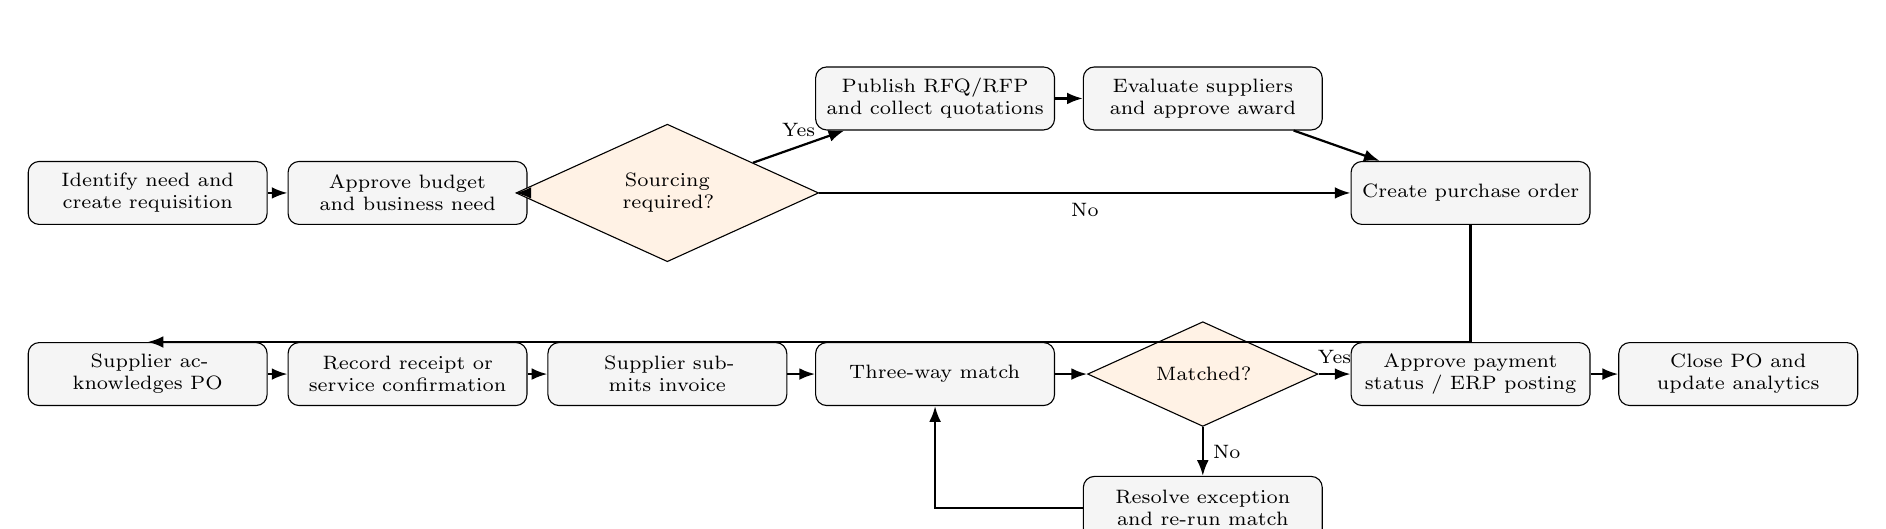
\begin{tikzpicture}[x=1cm,y=1cm]
  \node[act,text width=2.8cm] (need) at (-10,4) {Identify need and create requisition};
  \node[act,text width=2.8cm] (approve) at (-6.7,4) {Approve budget and business need};
  \node[decision,text width=2.0cm] (source) at (-3.4,4) {Sourcing required?};
  \node[act,text width=2.8cm] (rfq) at (0,5.2) {Publish RFQ/RFP and collect quotations};
  \node[act,text width=2.8cm] (eval) at (3.4,5.2) {Evaluate suppliers and approve award};
  \node[act,text width=2.8cm] (po) at (6.8,4) {Create purchase order};
  \node[act,text width=2.8cm] (ack) at (-10,1.7) {Supplier acknowledges PO};
  \node[act,text width=2.8cm] (receive) at (-6.7,1.7) {Record receipt or service confirmation};
  \node[act,text width=2.8cm] (invoice) at (-3.4,1.7) {Supplier submits invoice};
  \node[act,text width=2.8cm] (match) at (0,1.7) {Three-way match};
  \node[decision,text width=1.8cm] (ok) at (3.4,1.7) {Matched?};
  \node[act,text width=2.8cm] (pay) at (6.8,1.7) {Approve payment status / ERP posting};
  \node[act,text width=2.8cm] (close) at (10.2,1.7) {Close PO and update analytics};
  \node[act,text width=2.8cm] (except) at (3.4,0.0) {Resolve exception and re-run match};
  \draw[arrow] (need) -- (approve);
  \draw[arrow] (approve) -- (source);
  \draw[arrow] (source) -- node[above,font=\scriptsize]{Yes} (rfq);
  \draw[arrow] (rfq) -- (eval);
  \draw[arrow] (eval) -- (po);
  \draw[arrow] (source) -- node[below,font=\scriptsize]{No} (po);
  \draw[arrow] (po.south) |- (ack.north);
  \draw[arrow] (ack) -- (receive);
  \draw[arrow] (receive) -- (invoice);
  \draw[arrow] (invoice) -- (match);
  \draw[arrow] (match) -- (ok);
  \draw[arrow] (ok) -- node[above,font=\scriptsize]{Yes} (pay);
  \draw[arrow] (pay) -- (close);
  \draw[arrow] (ok) -- node[right,font=\scriptsize]{No} (except);
  \draw[arrow] (except.west) -| (match.south);
\end{tikzpicture}
\end{adjustbox}
\caption{Activity diagram - procurement workflow}
\end{figure}
\clearpage

\subsubsection{Activity A2 - Mudarabah capital application and approval}
\begin{figure}[h!]
\centering
\begin{adjustbox}{max width=1.05\linewidth}
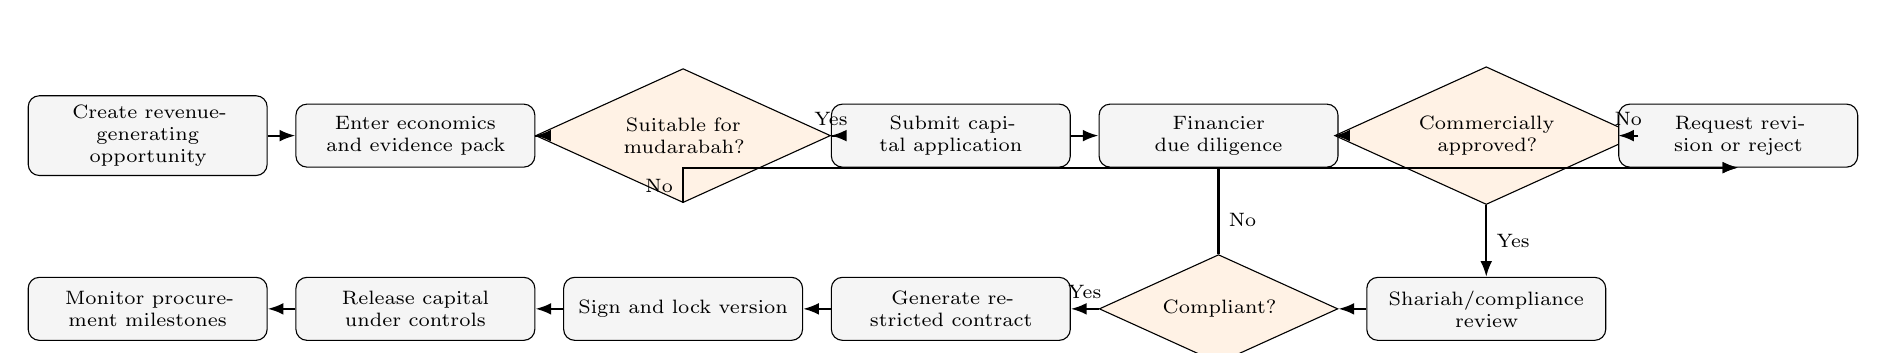
\begin{tikzpicture}[x=1cm,y=1cm]
  \node[act,text width=2.8cm] (opp) at (-10,4.5) {Create revenue-generating opportunity};
  \node[act,text width=2.8cm] (eco) at (-6.6,4.5) {Enter economics and evidence pack};
  \node[decision,text width=2.0cm] (suitable) at (-3.2,4.5) {Suitable for mudarabah?};
  \node[act,text width=2.8cm] (submit) at (0.2,4.5) {Submit capital application};
  \node[act,text width=2.8cm] (dd) at (3.6,4.5) {Financier due diligence};
  \node[decision,text width=2.0cm] (comm) at (7.0,4.5) {Commercially approved?};
  \node[act,text width=2.8cm] (revise) at (10.2,4.5) {Request revision or reject};
  \node[act,text width=2.8cm] (sh) at (7.0,2.3) {Shariah/compliance review};
  \node[decision,text width=1.8cm] (comp) at (3.6,2.3) {Compliant?};
  \node[act,text width=2.8cm] (contract) at (0.2,2.3) {Generate restricted contract};
  \node[act,text width=2.8cm] (sign) at (-3.2,2.3) {Sign and lock version};
  \node[act,text width=2.8cm] (disb) at (-6.6,2.3) {Release capital under controls};
  \node[act,text width=2.8cm] (mon) at (-10,2.3) {Monitor procurement milestones};
  \draw[arrow] (opp) -- (eco);
  \draw[arrow] (eco) -- (suitable);
  \draw[arrow] (suitable) -- node[above,font=\scriptsize]{Yes} (submit);
  \draw[arrow] (submit) -- (dd);
  \draw[arrow] (dd) -- (comm);
  \draw[arrow] (comm) -- node[above,font=\scriptsize]{No} (revise);
  \draw[arrow] (comm) -- node[right,font=\scriptsize]{Yes} (sh);
  \draw[arrow] (suitable.south) |- node[pos=.25,left,font=\scriptsize]{No} (revise.south);
  \draw[arrow] (sh) -- (comp);
  \draw[arrow] (comp) -- node[above,font=\scriptsize]{Yes} (contract);
  \draw[arrow] (comp.north) |- node[pos=.2,right,font=\scriptsize]{No} (revise.south);
  \draw[arrow] (contract) -- (sign);
  \draw[arrow] (sign) -- (disb);
  \draw[arrow] (disb) -- (mon);
\end{tikzpicture}
\end{adjustbox}
\caption{Activity diagram - mudarabah application and approval}
\end{figure}
\clearpage


\subsubsection{Activity A3 - Project monitoring, profit/loss, and closure}
\begin{figure}[h!]
\centering
\begin{adjustbox}{max width=1.05\linewidth}
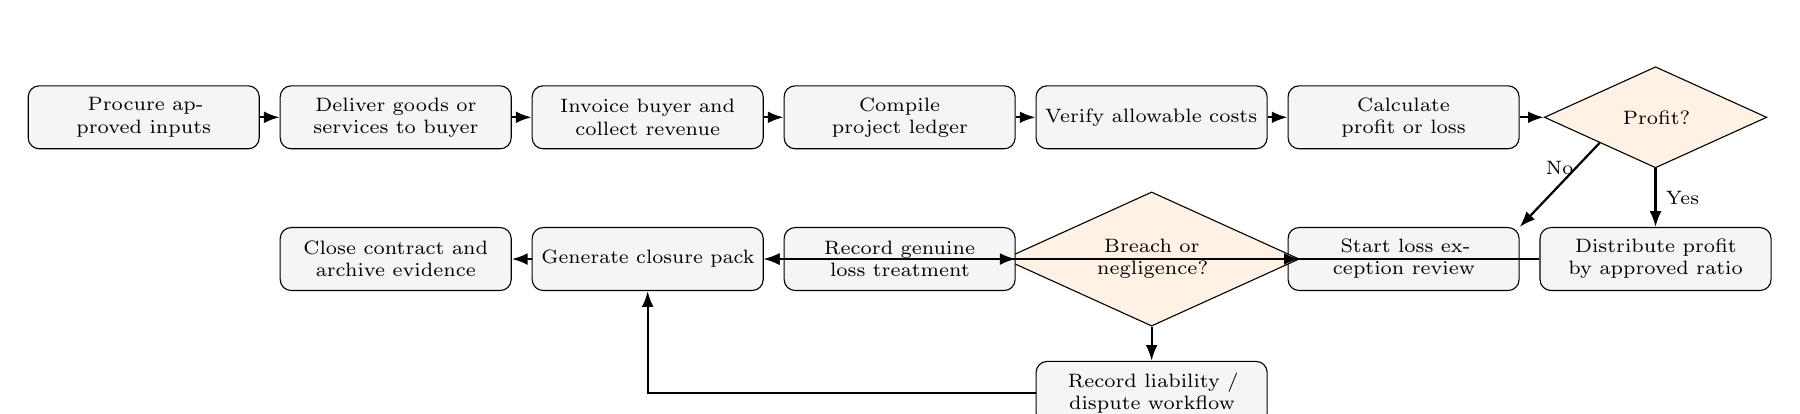
\begin{tikzpicture}[x=1cm,y=1cm]
  \node[act,text width=2.7cm] (exec) at (-10,4.4) {Procure approved inputs};
  \node[act,text width=2.7cm] (deliver) at (-6.8,4.4) {Deliver goods or services to buyer};
  \node[act,text width=2.7cm] (invoice) at (-3.6,4.4) {Invoice buyer and collect revenue};
  \node[act,text width=2.7cm] (ledger) at (-0.4,4.4) {Compile project ledger};
  \node[act,text width=2.7cm] (costs) at (2.8,4.4) {Verify allowable costs};
  \node[act,text width=2.7cm] (calc) at (6.0,4.4) {Calculate profit or loss};
  \node[decision,text width=1.7cm] (profit) at (9.2,4.4) {Profit?};
  \node[act,text width=2.7cm] (share) at (9.2,2.6) {Distribute profit by approved ratio};
  \node[act,text width=2.7cm] (review) at (6.0,2.6) {Start loss exception review};
  \node[decision,text width=1.9cm] (breach) at (2.8,2.6) {Breach or negligence?};
  \node[act,text width=2.7cm] (genuine) at (-0.4,2.6) {Record genuine loss treatment};
  \node[act,text width=2.7cm] (liability) at (2.8,0.9) {Record liability / dispute workflow};
  \node[act,text width=2.7cm] (close) at (-3.6,2.6) {Generate closure pack};
  \node[act,text width=2.7cm] (arch) at (-6.8,2.6) {Close contract and archive evidence};
  \draw[arrow] (exec.east) -- (deliver.west);
  \draw[arrow] (deliver.east) -- (invoice.west);
  \draw[arrow] (invoice.east) -- (ledger.west);
  \draw[arrow] (ledger.east) -- (costs.west);
  \draw[arrow] (costs.east) -- (calc.west);
  \draw[arrow] (calc.east) -- (profit.west);
  \draw[arrow] (profit.south) -- node[right,font=\scriptsize]{Yes} (share.north);
  \draw[arrow] (share.west) -- (close.east);
  \draw[arrow] (profit.south west) -- node[above,font=\scriptsize]{No} (review.north east);
  \draw[arrow] (review.west) -- (breach.east);
  \draw[arrow] (breach.west) -- (genuine.east);
  \draw[arrow] (breach.south) -- (liability.north);
  \draw[arrow] (genuine.west) -- (close.east);
  \draw[arrow] (liability.west) -| (close.south);
  \draw[arrow] (close.west) -- (arch.east);
\end{tikzpicture}
\end{adjustbox}
\caption{Activity diagram - mudarabah monitoring and closure}
\end{figure}
\clearpage

\subsubsection{Activity A4 - Supply-chain network canvas and audit anchoring}
\begin{figure}[h!]
\centering
\begin{adjustbox}{max width=1.05\linewidth}
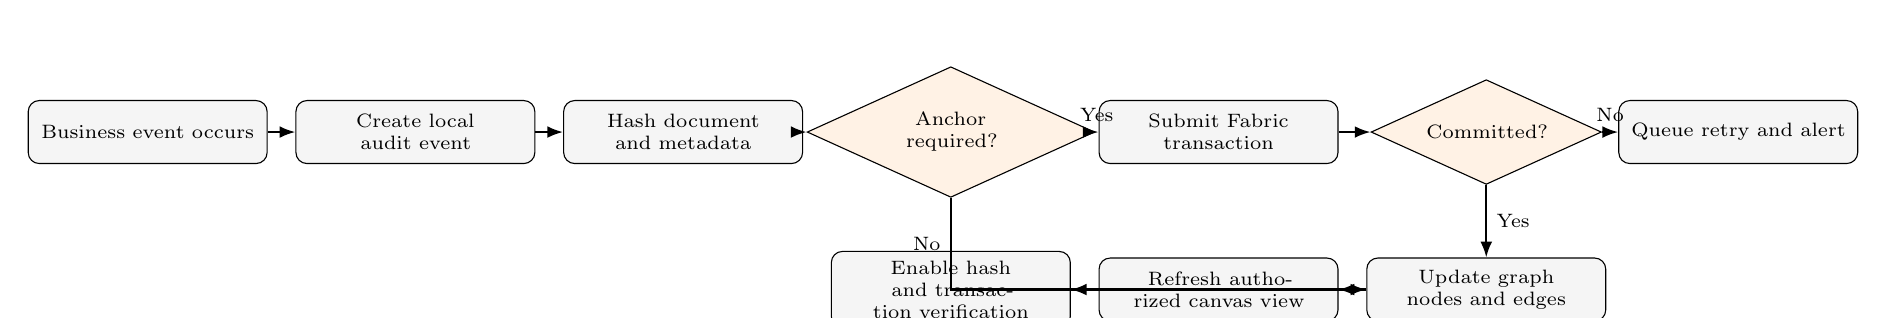
\begin{tikzpicture}[x=1cm,y=1cm]
  \node[act,text width=2.8cm] (event) at (-10,4) {Business event occurs};
  \node[act,text width=2.8cm] (audit) at (-6.6,4) {Create local audit event};
  \node[act,text width=2.8cm] (hash) at (-3.2,4) {Hash document and metadata};
  \node[decision,text width=1.8cm] (anchor) at (0.2,4) {Anchor required?};
  \node[act,text width=2.8cm] (fabric) at (3.6,4) {Submit Fabric transaction};
  \node[decision,text width=1.8cm] (commit) at (7.0,4) {Committed?};
  \node[act,text width=2.8cm] (retry) at (10.2,4) {Queue retry and alert};
  \node[act,text width=2.8cm] (graph) at (7.0,2) {Update graph nodes and edges};
  \node[act,text width=2.8cm] (view) at (3.6,2) {Refresh authorized canvas view};
  \node[act,text width=2.8cm] (verify) at (0.2,2) {Enable hash and transaction verification};
  \draw[arrow] (event) -- (audit);
  \draw[arrow] (audit) -- (hash);
  \draw[arrow] (hash) -- (anchor);
  \draw[arrow] (anchor) -- node[above,font=\scriptsize]{Yes} (fabric);
  \draw[arrow] (fabric) -- (commit);
  \draw[arrow] (commit) -- node[above,font=\scriptsize]{No} (retry);
  \draw[arrow] (commit) -- node[right,font=\scriptsize]{Yes} (graph);
  \draw[arrow] (anchor) |- node[pos=.25,left,font=\scriptsize]{No} (graph);
  \draw[arrow] (graph) -- (view);
  \draw[arrow] (view) -- (verify);
\end{tikzpicture}
\end{adjustbox}
\caption{Activity diagram - network canvas and audit anchoring}
\end{figure}
\end{landscape}
\clearpage


\begin{landscape}
\subsection{Domain Class Diagram}
\begin{figure}[h!]
\centering
\begin{adjustbox}{max width=1.05\linewidth}
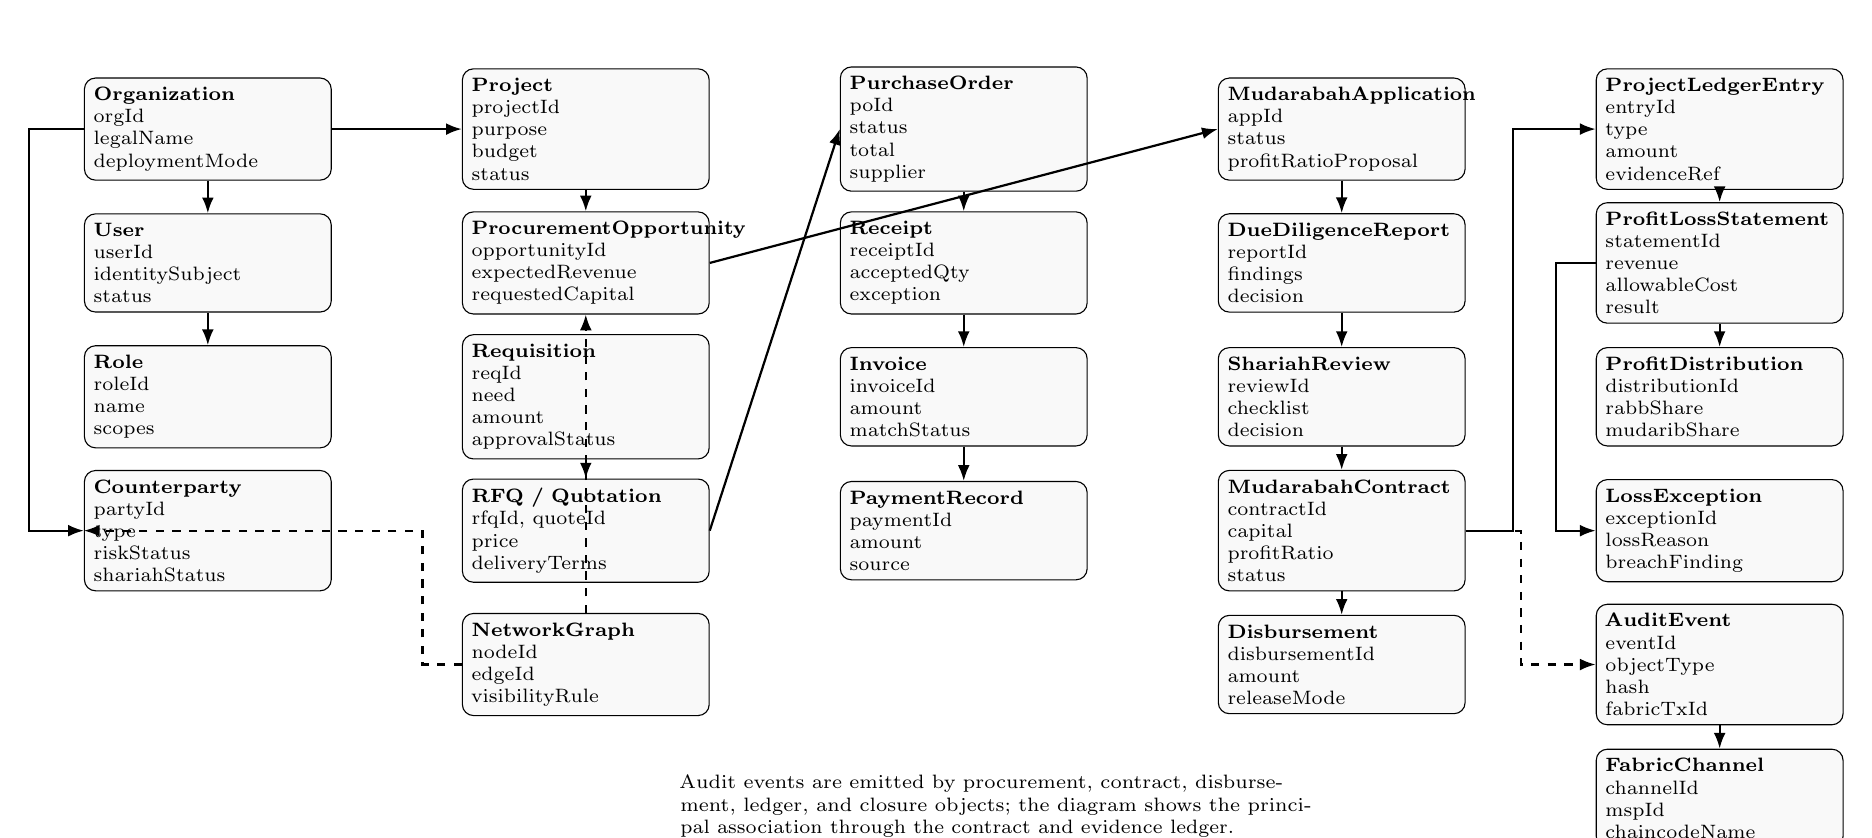
\begin{tikzpicture}[x=1cm,y=1cm]
  \node[classbox,text width=2.9cm] (org) at (-10,4.6) {\textbf{Organization}\par orgId\par legalName\par deploymentMode};
  \node[classbox,text width=2.9cm] (user) at (-10,2.9) {\textbf{User}\par userId\par identitySubject\par status};
  \node[classbox,text width=2.9cm] (role) at (-10,1.2) {\textbf{Role}\par roleId\par name\par scopes};
  \node[classbox,text width=2.9cm] (party) at (-10,-0.5) {\textbf{Counterparty}\par partyId\par type\par riskStatus\par shariahStatus};

  \node[classbox,text width=2.9cm] (project) at (-5.2,4.6) {\textbf{Project}\par projectId\par purpose\par budget\par status};
  \node[classbox,text width=2.9cm] (opp) at (-5.2,2.9) {\textbf{ProcurementOpportunity}\par opportunityId\par expectedRevenue\par requestedCapital};
  \node[classbox,text width=2.9cm] (req) at (-5.2,1.2) {\textbf{Requisition}\par reqId\par need\par amount\par approvalStatus};
  \node[classbox,text width=2.9cm] (rfq) at (-5.2,-0.5) {\textbf{RFQ / Quotation}\par rfqId, quoteId\par price\par deliveryTerms};
  \node[classbox,text width=2.9cm] (graph) at (-5.2,-2.2) {\textbf{NetworkGraph}\par nodeId\par edgeId\par visibilityRule};

  \node[classbox,text width=2.9cm] (po) at (-0.4,4.6) {\textbf{PurchaseOrder}\par poId\par status\par total\par supplier};
  \node[classbox,text width=2.9cm] (receipt) at (-0.4,2.9) {\textbf{Receipt}\par receiptId\par acceptedQty\par exception};
  \node[classbox,text width=2.9cm] (invoice) at (-0.4,1.2) {\textbf{Invoice}\par invoiceId\par amount\par matchStatus};
  \node[classbox,text width=2.9cm] (payment) at (-0.4,-0.5) {\textbf{PaymentRecord}\par paymentId\par amount\par source};

  \node[classbox,text width=2.9cm] (app) at (4.4,4.6) {\textbf{MudarabahApplication}\par appId\par status\par profitRatioProposal};
  \node[classbox,text width=2.9cm] (dd) at (4.4,2.9) {\textbf{DueDiligenceReport}\par reportId\par findings\par decision};
  \node[classbox,text width=2.9cm] (shr) at (4.4,1.2) {\textbf{ShariahReview}\par reviewId\par checklist\par decision};
  \node[classbox,text width=2.9cm] (contract) at (4.4,-0.5) {\textbf{MudarabahContract}\par contractId\par capital\par profitRatio\par status};
  \node[classbox,text width=2.9cm] (disb) at (4.4,-2.2) {\textbf{Disbursement}\par disbursementId\par amount\par releaseMode};

  \node[classbox,text width=2.9cm] (ledger) at (9.2,4.6) {\textbf{ProjectLedgerEntry}\par entryId\par type\par amount\par evidenceRef};
  \node[classbox,text width=2.9cm] (pl) at (9.2,2.9) {\textbf{ProfitLossStatement}\par statementId\par revenue\par allowableCost\par result};
  \node[classbox,text width=2.9cm] (dist) at (9.2,1.2) {\textbf{ProfitDistribution}\par distributionId\par rabbShare\par mudaribShare};
  \node[classbox,text width=2.9cm] (loss) at (9.2,-0.5) {\textbf{LossException}\par exceptionId\par lossReason\par breachFinding};
  \node[classbox,text width=2.9cm] (audit) at (9.2,-2.2) {\textbf{AuditEvent}\par eventId\par objectType\par hash\par fabricTxId};
  \node[classbox,text width=2.9cm] (fabric) at (9.2,-3.9) {\textbf{FabricChannel}\par channelId\par mspId\par chaincodeName};

  \draw[arrow] (org.south) -- (user.north);
  \draw[arrow] (user.south) -- (role.north);
  \draw[arrow] (org.west) -- ++(-0.7,0) |- (party.west);
  \draw[arrow] (org.east) -- (project.west);
  \draw[arrow] (project.south) -- (opp.north);
  \draw[arrow] (req.south) -- (rfq.north);
  \draw[arrow] (rfq.east) -- (po.west);
  \draw[arrow] (po.south) -- (receipt.north);
  \draw[arrow] (receipt.south) -- (invoice.north);
  \draw[arrow] (invoice.south) -- (payment.north);
  \draw[arrow] (opp.east) -- (app.west);
  \draw[arrow] (app.south) -- (dd.north);
  \draw[arrow] (dd.south) -- (shr.north);
  \draw[arrow] (shr.south) -- (contract.north);
  \draw[arrow] (contract.south) -- (disb.north);
  \draw[arrow] (contract.east) -- ++(0.6,0) |- (ledger.west);
  \draw[arrow] (ledger.south) -- (pl.north);
  \draw[arrow] (pl.south) -- (dist.north);
  \draw[arrow] (pl.west) -- ++(-0.5,0) |- (loss.west);
  \draw[arrow] (audit.south) -- (fabric.north);
  \draw[dashedarrow] (graph.west) -- ++(-0.5,0) |- (party.west);
  \draw[dashedarrow] (graph.north) -- (opp.south);
  \draw[dashedarrow] (contract.east) -- ++(0.7,0) |- (audit.west);
  \node[font=\scriptsize, align=left, text width=8cm] at (0,-4.0)
    {Audit events are emitted by procurement, contract, disbursement, ledger, and closure objects; the diagram shows the principal association through the contract and evidence ledger.};
\end{tikzpicture}
\end{adjustbox}
\caption{Domain class diagram showing principal classes and associations}
\end{figure}
\end{landscape}
\clearpage


\begin{landscape}
\subsection{State Machine Diagram - Mudarabah Contract Lifecycle}
The mudarabah contract lifecycle matters because capital release, loss treatment, auditability, and Shariah/compliance controls depend on state transitions. The diagram applies to the combined application-contract lifecycle.

\begin{figure}[h!]
\centering
\begin{adjustbox}{max width=1.05\linewidth}
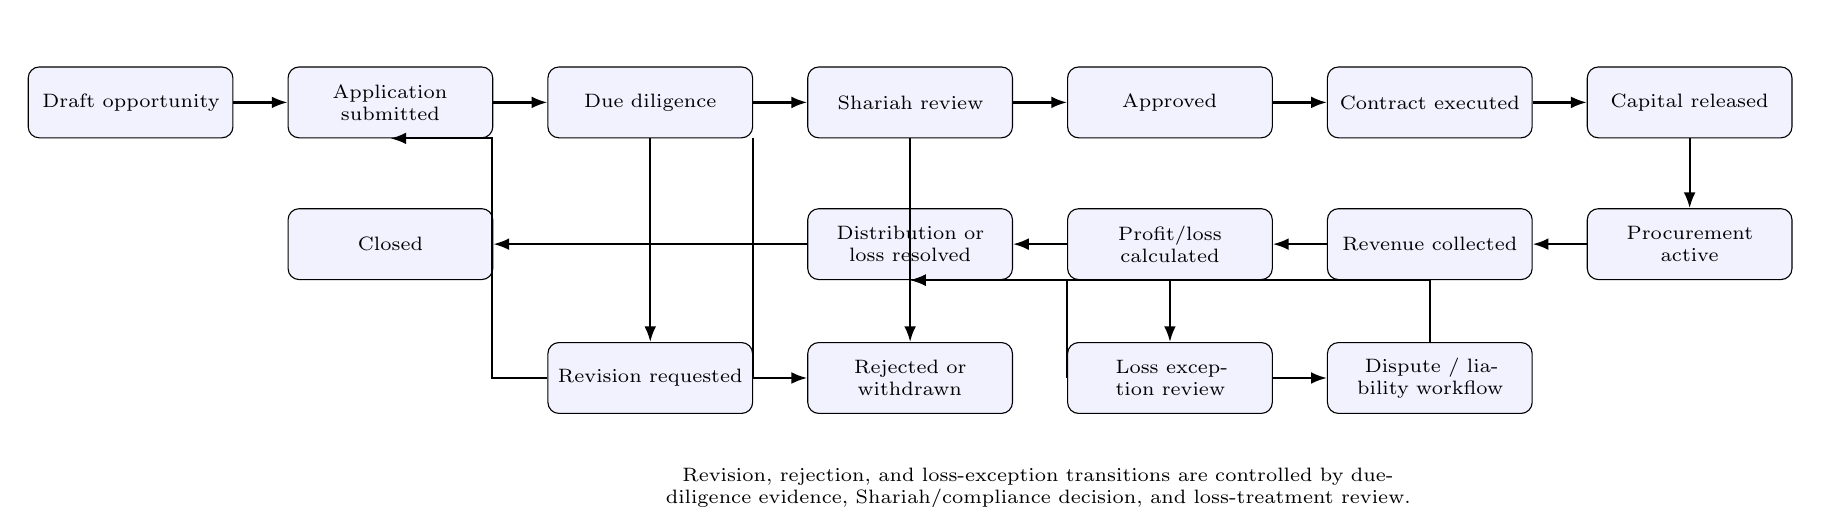
\begin{tikzpicture}[x=1cm,y=1cm]
  \node[state,minimum width=2.6cm,text width=2.35cm] (draft) at (-10.0,4.2) {Draft opportunity};
  \node[state,minimum width=2.6cm,text width=2.35cm] (submitted) at (-6.7,4.2) {Application submitted};
  \node[state,minimum width=2.6cm,text width=2.35cm] (dd) at (-3.4,4.2) {Due diligence};
  \node[state,minimum width=2.6cm,text width=2.35cm] (sh) at (-0.1,4.2) {Shariah review};
  \node[state,minimum width=2.6cm,text width=2.35cm] (approved) at (3.2,4.2) {Approved};
  \node[state,minimum width=2.6cm,text width=2.35cm] (executed) at (6.5,4.2) {Contract executed};
  \node[state,minimum width=2.6cm,text width=2.35cm] (released) at (9.8,4.2) {Capital released};
  \node[state,minimum width=2.6cm,text width=2.35cm] (active) at (9.8,2.4) {Procurement active};
  \node[state,minimum width=2.6cm,text width=2.35cm] (revenue) at (6.5,2.4) {Revenue collected};
  \node[state,minimum width=2.6cm,text width=2.35cm] (pl) at (3.2,2.4) {Profit/loss calculated};
  \node[state,minimum width=2.6cm,text width=2.35cm] (resolved) at (-0.1,2.4) {Distribution or loss resolved};
  \node[state,minimum width=2.6cm,text width=2.35cm] (closed) at (-6.7,2.4) {Closed};
  \node[state,minimum width=2.6cm,text width=2.35cm] (revision) at (-3.4,0.7) {Revision requested};
  \node[state,minimum width=2.6cm,text width=2.35cm] (rejected) at (-0.1,0.7) {Rejected or withdrawn};
  \node[state,minimum width=2.6cm,text width=2.35cm] (exception) at (3.2,0.7) {Loss exception review};
  \node[state,minimum width=2.6cm,text width=2.35cm] (dispute) at (6.5,0.7) {Dispute / liability workflow};

  \draw[arrow] (draft.east) -- (submitted.west);
  \draw[arrow] (submitted.east) -- (dd.west);
  \draw[arrow] (dd.east) -- (sh.west);
  \draw[arrow] (sh.east) -- (approved.west);
  \draw[arrow] (approved.east) -- (executed.west);
  \draw[arrow] (executed.east) -- (released.west);
  \draw[arrow] (released.south) -- (active.north);
  \draw[arrow] (active.west) -- (revenue.east);
  \draw[arrow] (revenue.west) -- (pl.east);
  \draw[arrow] (pl.west) -- (resolved.east);
  \draw[arrow] (resolved.west) -- (closed.east);
  \draw[arrow] (dd.south) -- (revision.north);
  \draw[arrow] (revision.west) -- ++(-0.7,0) |- (submitted.south);
  \draw[arrow] (sh.south) -- (rejected.north);
  \draw[arrow] (dd.south east) |- (rejected.west);
  \draw[arrow] (pl.south) -- (exception.north);
  \draw[arrow] (exception.east) -- (dispute.west);
  \draw[arrow] (exception.west) |- (resolved.south);
  \draw[arrow] (dispute.north) |- (resolved.south);
  \node[font=\scriptsize, align=center, text width=15cm] at (1.5,-0.7) {Revision, rejection, and loss-exception transitions are controlled by due-diligence evidence, Shariah/compliance decision, and loss-treatment review.};
\end{tikzpicture}
\end{adjustbox}
\caption{State machine - mudarabah application and contract lifecycle}
\end{figure}
\end{landscape}
\clearpage

\subsection{Sequence Diagrams for External Integrations}
Sequence diagrams are included only where \systemshort{} interacts with external systems.

\subsubsection{Sequence S1 - OAuth/OIDC login}
\begin{figure}[h]
\centering
\begin{adjustbox}{max width=\textwidth}
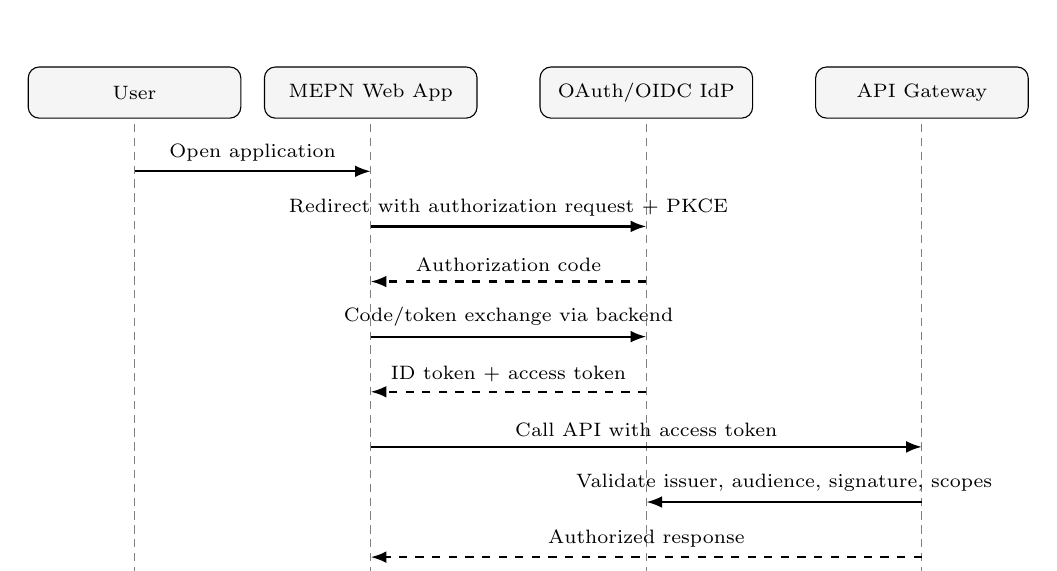
\begin{tikzpicture}[x=1cm,y=1cm]
  \node[seqnode] (u) at (0,0) {User};
  \node[seqnode] (web) at (3,0) {MEPN Web App};
  \node[seqnode] (idp) at (6.5,0) {OAuth/OIDC IdP};
  \node[seqnode] (api) at (10,0) {API Gateway};
  \foreach \x in {0,3,6.5,10} {\draw[lifeline] (\x,-0.4) -- (\x,-6.2);}
  \draw[msg] (0,-1) -- node[above]{Open application} (3,-1);
  \draw[msg] (3,-1.7) -- node[above]{Redirect with authorization request + PKCE} (6.5,-1.7);
  \draw[returnmsg] (6.5,-2.4) -- node[above]{Authorization code} (3,-2.4);
  \draw[msg] (3,-3.1) -- node[above]{Code/token exchange via backend} (6.5,-3.1);
  \draw[returnmsg] (6.5,-3.8) -- node[above]{ID token + access token} (3,-3.8);
  \draw[msg] (3,-4.5) -- node[above]{Call API with access token} (10,-4.5);
  \draw[msg] (10,-5.2) -- node[above]{Validate issuer, audience, signature, scopes} (6.5,-5.2);
  \draw[returnmsg] (10,-5.9) -- node[above]{Authorized response} (3,-5.9);
\end{tikzpicture}
\end{adjustbox}
\caption{Sequence diagram - OAuth/OIDC login}
\end{figure}

\subsubsection{Sequence S2 - ERP synchronization}
\begin{figure}[h]
\centering
\begin{adjustbox}{max width=\textwidth}
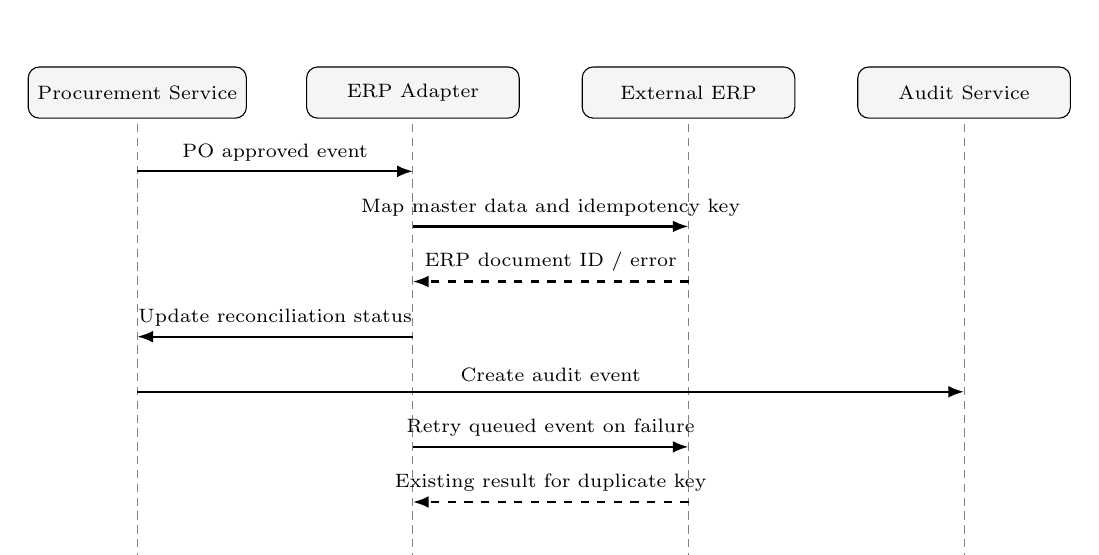
\begin{tikzpicture}[x=1cm,y=1cm]
  \node[seqnode] at (0,0) {Procurement Service};
  \node[seqnode] at (3.5,0) {ERP Adapter};
  \node[seqnode] at (7,0) {External ERP};
  \node[seqnode] at (10.5,0) {Audit Service};
  \foreach \x in {0,3.5,7,10.5} {\draw[lifeline] (\x,-0.4) -- (\x,-6.0);}
  \draw[msg] (0,-1) -- node[above]{PO approved event} (3.5,-1);
  \draw[msg] (3.5,-1.7) -- node[above]{Map master data and idempotency key} (7,-1.7);
  \draw[returnmsg] (7,-2.4) -- node[above]{ERP document ID / error} (3.5,-2.4);
  \draw[msg] (3.5,-3.1) -- node[above]{Update reconciliation status} (0,-3.1);
  \draw[msg] (0,-3.8) -- node[above]{Create audit event} (10.5,-3.8);
  \draw[msg] (3.5,-4.5) -- node[above]{Retry queued event on failure} (7,-4.5);
  \draw[returnmsg] (7,-5.2) -- node[above]{Existing result for duplicate key} (3.5,-5.2);
\end{tikzpicture}
\end{adjustbox}
\caption{Sequence diagram - external ERP integration}
\end{figure}

\subsubsection{Sequence S3 - Hyperledger Fabric event anchoring}
\begin{figure}[h]
\centering
\begin{adjustbox}{max width=\textwidth}
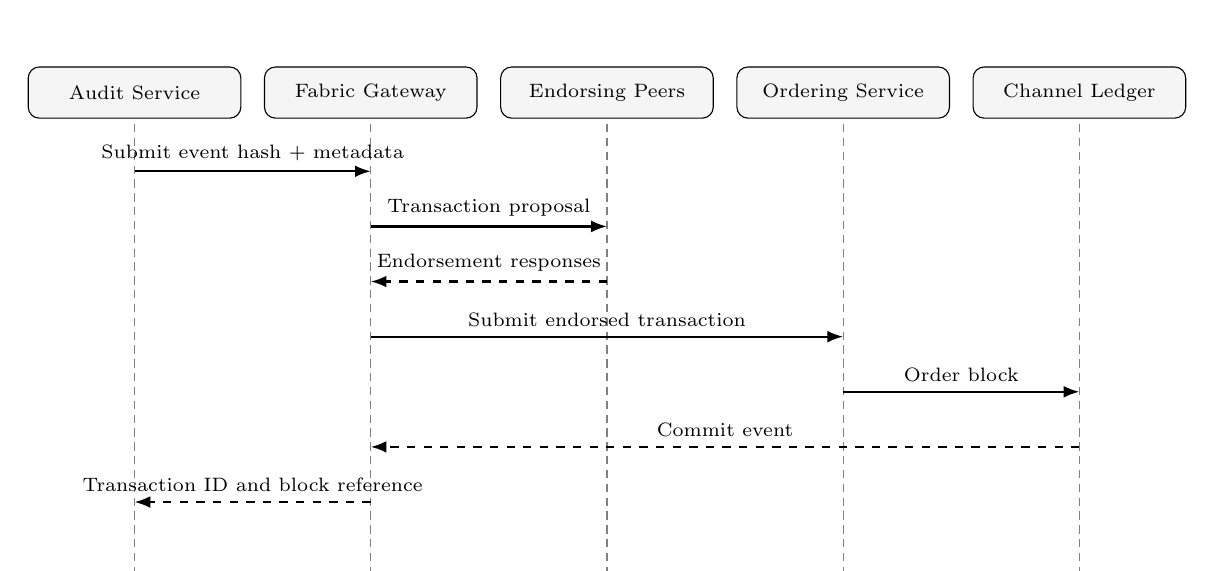
\begin{tikzpicture}[x=1cm,y=1cm]
  \node[seqnode] at (0,0) {Audit Service};
  \node[seqnode] at (3,0) {Fabric Gateway};
  \node[seqnode] at (6,0) {Endorsing Peers};
  \node[seqnode] at (9,0) {Ordering Service};
  \node[seqnode] at (12,0) {Channel Ledger};
  \foreach \x in {0,3,6,9,12} {\draw[lifeline] (\x,-0.4) -- (\x,-6.2);}
  \draw[msg] (0,-1) -- node[above]{Submit event hash + metadata} (3,-1);
  \draw[msg] (3,-1.7) -- node[above]{Transaction proposal} (6,-1.7);
  \draw[returnmsg] (6,-2.4) -- node[above]{Endorsement responses} (3,-2.4);
  \draw[msg] (3,-3.1) -- node[above]{Submit endorsed transaction} (9,-3.1);
  \draw[msg] (9,-3.8) -- node[above]{Order block} (12,-3.8);
  \draw[returnmsg] (12,-4.5) -- node[above]{Commit event} (3,-4.5);
  \draw[returnmsg] (3,-5.2) -- node[above]{Transaction ID and block reference} (0,-5.2);
\end{tikzpicture}
\end{adjustbox}
\caption{Sequence diagram - Fabric event anchoring}
\end{figure}

\subsubsection{Sequence S4 - Financial entity disbursement API}
\begin{figure}[h]
\centering
\begin{adjustbox}{max width=\textwidth}
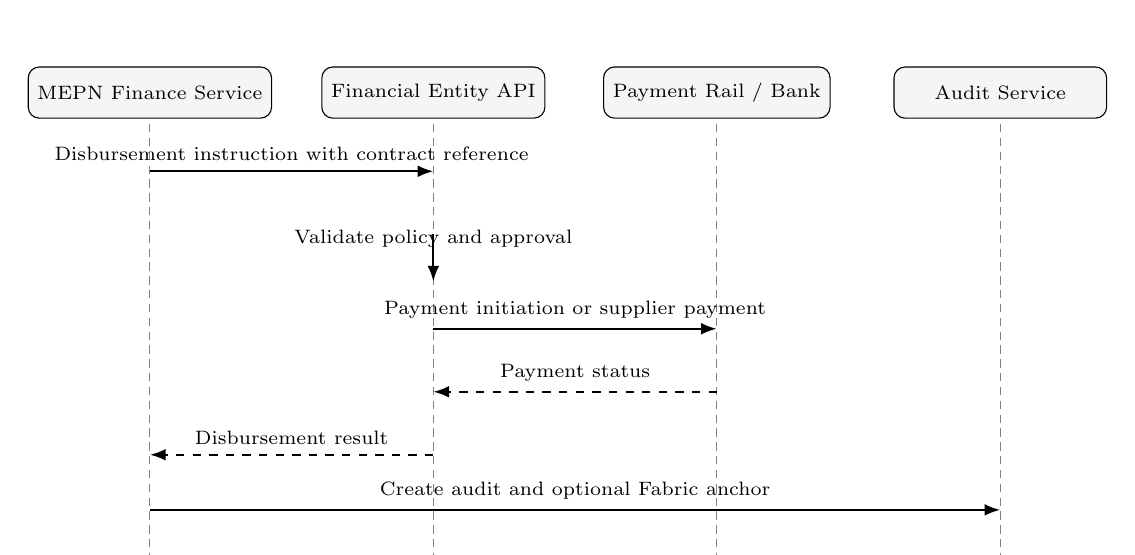
\begin{tikzpicture}[x=1cm,y=1cm]
  \node[seqnode] at (0,0) {MEPN Finance Service};
  \node[seqnode] at (3.6,0) {Financial Entity API};
  \node[seqnode] at (7.2,0) {Payment Rail / Bank};
  \node[seqnode] at (10.8,0) {Audit Service};
  \foreach \x in {0,3.6,7.2,10.8} {\draw[lifeline] (\x,-0.4) -- (\x,-6.0);}
  \draw[msg] (0,-1) -- node[above]{Disbursement instruction with contract reference} (3.6,-1);
  \draw[msg] (3.6,-1.8) -- node[above]{Validate policy and approval} (3.6,-2.4);
  \draw[msg] (3.6,-3.0) -- node[above]{Payment initiation or supplier payment} (7.2,-3.0);
  \draw[returnmsg] (7.2,-3.8) -- node[above]{Payment status} (3.6,-3.8);
  \draw[returnmsg] (3.6,-4.6) -- node[above]{Disbursement result} (0,-4.6);
  \draw[msg] (0,-5.3) -- node[above]{Create audit and optional Fabric anchor} (10.8,-5.3);
\end{tikzpicture}
\end{adjustbox}
\caption{Sequence diagram - external financial entity disbursement API}
\end{figure}

\section{Verification Plan}

\subsection{Verification strategy}
Verification shall be organized by requirement class and release stage. P0 requirements shall be verified before MVP acceptance. P1 requirements shall be verified before commercial beta. P2 requirements shall be verified before optional release activation. Every verification record shall link to the requirement ID, test artifact, tester/reviewer, date, input data, result, evidence, and defect reference where applicable.

\subsection{Verification coverage by requirement group}
\begin{table}[h]
\centering
\begin{tabularx}{\textwidth}{@{}p{0.23\textwidth}X@{}}
\toprule
Requirement group & Minimum verification evidence \\
\midrule
Identity and authorization & Token validation tests, role matrix tests, unauthorized access attempts, audit log inspection. \\
Procurement workflow & Scenario tests for requisition, RFQ, quotation, PO, receipt, invoice, match exception, payment status, and closure. \\
Mudarabah finance & Scenario tests for application completeness, due diligence, Shariah review, contract generation, disbursement, project ledger, profit/loss, and loss exception. \\
ERP integration & Adapter mapping tests, idempotency tests, duplicate handling, reconciliation status, and failure retry tests. \\
Fabric integration & Chaincode transaction tests, event hash verification, failed gateway retry, transaction ID recording, API-side \code{ReadAnchor} verification, and channel access control. \\
Fabric governance & Metadata, proposal, invitation, approval, readiness, operator execution, sanitized evidence, and no-admin-secret custody tests. \\
Network canvas & Graph permission tests, filter/search tests, saved-view tests, annotation target visibility tests, redaction tests, and no-leak browser tests. \\
Security and audit & Penetration-oriented test cases, secrets inspection, TLS checks, immutable audit log checks, and contract amendment workflow tests. \\
Deployment and operations & Installation test, migration test, backup/restore test, health/readiness check, worker heartbeat, operations timeline, observability review, and upgrade rollback rehearsal. \\
\bottomrule
\end{tabularx}
\caption{Verification coverage summary}
\end{table}

\subsection{Acceptance criteria for MVP}
The MVP shall not be accepted unless all P0 requirements are either passed or formally waived by the product owner, system owner, and risk owner. Waivers for Shariah, legal, security, or financial control requirements shall require documented reviewer sign-off and expiry date.

For the current FYP review baseline, acceptance evidence is recorded in the evidence index and final validation matrix. Evidence must distinguish implemented review-scope behavior from production-hardening work and must not treat mock integrations, seeded data, or locally stored metadata as real external proof.

\section{Traceability Matrix}
\begin{landscape}
\begin{footnotesize}
\begin{longtable}{@{}p{0.08\linewidth}p{0.16\linewidth}p{0.14\linewidth}p{0.22\linewidth}p{0.14\linewidth}p{0.16\linewidth}@{}}
\rowcolor{gray!18}\textbf{Need} & \textbf{Need summary} & \textbf{Business reqs} & \textbf{Software reqs} & \textbf{UML coverage} & \textbf{Verification evidence} \\ \hline
\endfirsthead
\rowcolor{gray!18}\textbf{Need} & \textbf{Need summary} & \textbf{Business reqs} & \textbf{Software reqs} & \textbf{UML coverage} & \textbf{Verification evidence} \\ \hline
\endhead
SN-01 & SME-controlled e-procurement & BR-01, BR-05 & FR-01 to FR-24, IR-05 to IR-07, NFR-19 & UC-01, UC-04, UC-05, UC-15 & Test, demonstration, install test \\ \hline
SN-02 & Working capital for procurement opportunities & BR-02, BR-06 & FR-25 to FR-28, FR-34 & UC-06, UC-07, UC-10 & Scenario test, review \\ \hline
SN-03 & Reduce financier information asymmetry & BR-03, BR-04, BR-08 & FR-28 to FR-42, DR-02, DR-07 & UC-07 to UC-12 & Due diligence review, evidence pack inspection \\ \hline
SN-04 & Monitoring without management takeover & BR-03, BR-07 & FR-35, FR-36, FR-40, FR-47 to FR-50 & UC-11, UC-14 & Dashboard demo, audit verification \\ \hline
SN-05 & Shariah and compliance governance & BR-03, BR-04 & FR-30 to FR-32, FR-38, FR-39 & UC-09, UC-12 & Reviewer acceptance, workflow test \\ \hline
SN-06 & Supply-chain network visibility & BR-09 & FR-43 to FR-46, DR-09 & UC-13 & Canvas demo, permission test \\ \hline
SN-07 & ERP/accounting integration & BR-01, BR-03 & IR-05 to IR-07, FR-36, DR-07, NFR-11 & UC-05, UC-15 & Integration test, reconciliation test \\ \hline
SN-08 & Tamper-evident auditability & BR-03, BR-07, BR-08 & FR-47 to FR-50, DR-04, DR-05, NFR-09 & UC-10, UC-11, UC-14 & Fabric test, audit inspection \\ \hline
SN-09 & Installable SME deployment & BR-05 & FR-01, NFR-10, NFR-13, NFR-19, NFR-20 & UC-01 & Install, backup, restore, health check \\ \hline
SN-10 & Future feature extension & BR-10 & FR-52, IR-01, IR-12, DR-10, NFR-24 & UC-01, UC-15 & API inspection, plugin sandbox review \\ \hline
SN-11 & Reviewer-safe operations evidence & BR-11 & FR-56, DR-11, NFR-06, NFR-10, NFR-13, NFR-19 & UC-01, UC-14 & Operations timeline, backup/restore, deployment evidence \\ \hline
SN-12 & Operator-assisted Fabric governance & BR-12 & FR-55, IR-13, DR-12, NFR-06, NFR-18 & UC-01, UC-14 & Fabric governance workflow tests and evidence inspection \\ \hline

\end{longtable}
\end{footnotesize}
\end{landscape}

\appendix
\section{Assumptions and Dependencies}

\subsection{Assumptions}
\begin{enumerate}
  \item SMEs will operate the system for revenue-generating procurement opportunities where project-level profit/loss can be measured.
  \item Financial entities will define underwriting policies, reviewer roles, product limits, disbursement controls, and Shariah requirements.
  \item At least one deployment mode will be available for SMEs with limited IT resources through Docker Compose.
  \item Fabric channel governance for the current baseline is operator-assisted. Any future automated channel topology mutation requires a separate secret-custody, managed-operator, and recovery decision.
  \item ERP integration will vary by SME maturity; CSV/XLSX exchange is therefore retained as a fallback.
  \item Legal enforceability, Shariah approval, accounting treatment, and regulatory reporting requirements will be finalized per jurisdiction and institution.
\end{enumerate}

\subsection{Dependencies}
\begin{itemize}
  \item OAuth/OIDC identity provider or bundled identity component.
  \item PostgreSQL, object storage, queue/cache, email provider, and backup storage.
  \item Hyperledger Fabric gateway, channel configuration, MSP identity material, and approved chaincode for audit anchors; Fabric admin identities for channel topology changes are explicitly outside the current application runtime.
  \item ERP/accounting APIs or import/export capabilities.
  \item Optional e-signature provider, payment rail, banking API, and financial entity workflow API.
  \item Legal, Shariah, accounting, cybersecurity, and data protection review before production release.
\end{itemize}

\section{Acronyms and Abbreviations}
\begin{longtable}{@{}p{0.20\textwidth}p{0.75\textwidth}@{}}
\rowcolor{gray!18}\textbf{Acronym} & \textbf{Meaning} \\ \hline
API & Application Programming Interface \\ \hline
ERP & Enterprise Resource Planning \\ \hline
IdP & Identity Provider \\ \hline
MEPN & Mudarabah-Enabled Procurement Network \\ \hline
MSP & Membership Service Provider in Hyperledger Fabric \\ \hline
OIDC & OpenID Connect \\ \hline
P2P & Procure-to-pay \\ \hline
PO & Purchase Order \\ \hline
RBAC & Role-Based Access Control \\ \hline
RFQ/RFP/RFI & Request for Quotation / Proposal / Information \\ \hline
RTM & Requirements Traceability Matrix \\ \hline
S2C & Source-to-contract \\ \hline
SME & Small and Medium Enterprise \\ \hline
SRS & Software Requirements Specification \\ \hline
TLS & Transport Layer Security \\ \hline
UML & Unified Modeling Language \\ \hline
\end{longtable}

\section{Open Issues for Product Discovery}
\begin{longtable}{@{}p{0.12\textwidth}p{0.65\textwidth}p{0.18\textwidth}@{}}
\rowcolor{gray!18}\textbf{ID} & \textbf{Issue} & \textbf{Owner} \\ \hline
OI-01 & Select the first target jurisdiction and map legal/Shariah/regulatory requirements to production controls. & Product + Legal/Shariah \\ \hline
OI-02 & Decide whether the financial entity portal is always self-hosted by the financier or can be hosted by an SME consortium operator. & Product Architecture \\ \hline
OI-03 & Define minimum borrower accounting maturity required for live mudarabah financing. & Finance/Risk \\ \hline
OI-04 & Select initial ERP adapters and document canonical field mappings. & Integration Team \\ \hline
OI-05 & Decide if and when operator-assisted Fabric governance should evolve into automated topology administration, including managed secret store, operator-agent, signing, retry, and recovery policies. & Product + Distributed Ledger + Security \\ \hline
OI-06 & Configure and verify a real production OIDC provider, invite-token policy, MFA/password policy, and provider-specific callback deployment behavior. & Product + Security \\ \hline
OI-07 & Define production PDF/spreadsheet report packs, retention rules, evidence-item registration, and regulatory-ready layouts. & Product + Compliance \\ \hline
OI-08 & Prioritize future discovered features such as AI-assisted risk scoring, anomaly detection, negotiation support, or automated document extraction. & Product Owner \\ \hline
\end{longtable}

\section{Conformance Notes}
This document is intended as a requirements specification artifact aligned with ISO/IEC/IEEE 29148 content guidance. It does not assert that the complete project lifecycle, organizational process, or all information items have achieved full standard conformance. It establishes a requirements baseline that can be reviewed, changed, and traced through formal requirements management.

\end{document}
